\documentclass[12pt,a4paper]{article}
\usepackage[a4paper, margin=0.8in, headheight=14pt]{geometry}
\usepackage{fontspec}
\usepackage{unicode-math}
\setmainfont{TeX Gyre Pagella}
\setmonofont[Scale=0.88]{TeX Gyre Cursor}
\setmathfont{Latin Modern Math}
\usepackage{xcolor}
\usepackage{titlesec}
\usepackage{enumitem}
\usepackage{tabularx}
\usepackage{booktabs}
\usepackage{array}
\usepackage{amsmath}
\usepackage{tikz}
\usetikzlibrary{shapes.geometric, arrows.meta, positioning, calc, fit, decorations.pathreplacing}
\usepackage{tcolorbox}
\tcbuselibrary{skins, breakable}
\usepackage{hyperref}
\usepackage{fancyhdr}
\usepackage{graphicx}
\usepackage{microtype}
\hyphenpenalty=10000
\exhyphenpenalty=10000
\sloppy
\usepackage{caption}
\usepackage{setspace}
\usepackage{multirow}
\usepackage{tocloft}
\newcommand{\Q}[1]{\textbf{#1}\par\noindent\ignorespaces}
\definecolor{myred}{RGB}{196,30,58}
\definecolor{mydark}{RGB}{30,30,50}
\definecolor{mygreen}{RGB}{14,120,80}
\definecolor{myteal}{RGB}{0,130,140}
\definecolor{myamber}{RGB}{180,100,0}
\definecolor{mypurple}{RGB}{100,30,160}
\definecolor{mygray}{RGB}{246,247,249}
\definecolor{mgframe}{RGB}{180,185,200}
\definecolor{watermark}{RGB}{145,150,170}
\definecolor{hdrred}{RGB}{250,232,235}
\definecolor{hdrgreen}{RGB}{220,244,233}
\definecolor{hdrteal}{RGB}{220,242,244}
\definecolor{hdramber}{RGB}{253,242,215}
\definecolor{hdrpurple}{RGB}{238,228,255}
\definecolor{hdrgray}{RGB}{238,240,245}
\definecolor{rowalt}{RGB}{250,251,253}

\titleformat{\section}{\large\bfseries\color{myred}}{\thesection.}{0.5em}{}[\vspace{1pt}{\color{myred}\rule{\linewidth}{0.8pt}}]
\titleformat{\subsection}{\normalsize\bfseries\color{myteal}}{\thesubsection}{0.5em}{}
\titlespacing*{\section}{0pt}{18pt}{7pt}
\titlespacing*{\subsection}{0pt}{11pt}{4pt}
\setlength{\parindent}{0pt}
\setlength{\parskip}{4pt}
\renewcommand{\cfttoctitlefont}{\large\bfseries\color{myred}}
\renewcommand{\cftaftertoctitle}{\par\noindent{\color{myred}\rule{\linewidth}{0.8pt}}}
\setlength{\cftbeforetoctitleskip}{0pt}
\setlength{\cftaftertoctitleskip}{6pt}
\renewcommand{\cftsecfont}{\normalsize\bfseries\color{mydark}}
\renewcommand{\cftsecpagefont}{\normalsize\bfseries\color{mydark}}
\renewcommand{\cftsecleader}{\cftdotfill{\cftdotsep}}
\setlength{\cftbeforesecskip}{7pt}
\renewcommand{\cftsubsecfont}{\small\color{mydark}}
\renewcommand{\cftsubsecpagefont}{\small\color{mydark}}
\setlength{\cftbeforesubsecskip}{3pt}
\setlength{\cftsubsecindent}{1.4em}
\renewcommand{\cftpartfont}{\normalsize\bfseries\color{myteal}}
\renewcommand{\cftpartpagefont}{\normalsize\bfseries\color{myteal}}
\setlength{\cftbeforepartskip}{14pt}
\renewcommand{\arraystretch}{1.45}
\setlength{\tabcolsep}{6pt}
\newcolumntype{B}[1]{>{\small\bfseries\raggedright\arraybackslash}m{#1}}
\newcolumntype{C}[1]{>{\centering\arraybackslash}m{#1}}
\newcolumntype{Y}{>{\small\raggedright\arraybackslash}X}
\renewcommand{\tabularxcolumn}[1]{m{#1}}
\newcommand{\currmodule}{Module 1}
\pagestyle{fancy}
\fancyhf{}
\fancyhead[L]{\small\color{myred}\textbf{OE-EC604C}\;\color{mydark}--- Object Oriented Programming}
\fancyhead[R]{\small\color{myteal}\textbf{\currmodule\ Notes}}
\fancyfoot[C]{\small\color{mydark}\thepage}
\fancyfoot[R]{\small\color{watermark}\textit{\copyright\ Biraj}}
\renewcommand{\headrulewidth}{0.5pt}
\renewcommand{\footrulewidth}{0.3pt}

\hypersetup{colorlinks=true, linkcolor=myteal, urlcolor=myteal,
  pdfauthor={Biraj Sarkar},
  pdftitle={OE-EC604C --- Combined Notes}}

\tcbset{
  tikzbox/.style={
    colback=mygray, colframe=mgframe, boxrule=0.6pt, arc=4pt,
    left=8pt, right=8pt, top=6pt, bottom=6pt,
    colbacktitle=mgframe, coltitle=mydark,
    fonttitle=\small\bfseries
  },
  defbox/.style={
    colback=hdrgreen, colframe=mygreen, boxrule=0.8pt, arc=4pt,
    left=9pt, right=9pt, top=6pt, bottom=6pt,
    colbacktitle=mygreen, coltitle=white,
    fonttitle=\small\bfseries
  },
  formulabox/.style={
    colback=hdrteal, colframe=myteal, boxrule=0.8pt, arc=4pt,
    left=9pt, right=9pt, top=7pt, bottom=7pt,
    colbacktitle=myteal, coltitle=white,
    fonttitle=\small\bfseries
  },
  examplebox/.style={
    colback=hdramber, colframe=myamber, boxrule=0.8pt, arc=4pt,
    left=9pt, right=9pt, top=6pt, bottom=6pt,
    colbacktitle=myamber, coltitle=white,
    fonttitle=\small\bfseries
  },
  masonbox/.style={
    colback=hdrpurple, colframe=mypurple, boxrule=0.8pt, arc=4pt,
    left=9pt, right=9pt, top=6pt, bottom=6pt,
    colbacktitle=mypurple, coltitle=white,
    fonttitle=\small\bfseries
  },
  exambox/.style={
    colback=hdrpurple, colframe=mypurple, boxrule=1pt, arc=5pt,
    left=10pt, right=10pt, top=8pt, bottom=8pt,
    colbacktitle=mypurple, coltitle=white,
    fonttitle=\bfseries,
    breakable, title after break={\textbf{Frequently Asked / Viva Questions (contd.)}}}
}
\tcbset{breakable}

\tikzset{
  block/.style={rectangle, draw=myteal, fill=hdrteal,
    text width=2.4cm, align=center, minimum height=0.95cm,
    font=\small, rounded corners=3pt, line width=0.7pt},
  redblock/.style={rectangle, draw=myred, fill=hdrred,
    text width=2.4cm, align=center, minimum height=0.95cm,
    font=\small, rounded corners=3pt, line width=0.7pt},
  netnode/.style={rectangle, draw=myteal, fill=hdrteal,
    text width=1.5cm, align=center, minimum height=0.8cm,
    font=\small, rounded corners=3pt, line width=0.7pt},
  sumjunc/.style={circle, draw=myamber, fill=hdramber,
    minimum size=0.62cm, font=\small, line width=0.8pt},
  snode/.style={circle, draw=mypurple, fill=hdrpurple,
    minimum size=0.55cm, font=\footnotesize, line width=0.7pt},
  arrow/.style={-Stealth, thick, color=mydark},
  redarrow/.style={-Stealth, thick, color=myred},
  line/.style={thick, color=mydark}
}

\newcommand{\modulestart}[2]{%
  \clearpage
  \renewcommand{\currmodule}{Module #1}%
  \phantomsection
  \addcontentsline{toc}{part}{Module #1: #2}%
  \setcounter{section}{0}%
  \begin{center}
    \vspace*{1.0cm}
    {\Huge\bfseries\color{myred} Module #1}\\[10pt]
    {\Large\bfseries\color{mydark} #2}\\[10pt]
    {\color{myred}\rule{0.55\linewidth}{1.2pt}}
  \end{center}
  \vspace{14pt}
}
\begin{document}

\thispagestyle{empty}
\vspace*{1.0cm}
\begin{center}
  {\Huge\bfseries\color{myred} OE-EC604C}\\[10pt]
  {\LARGE\bfseries\color{mydark} Object Oriented Programming}\\[20pt]
  {\color{myred}\rule{0.7\linewidth}{1.5pt}}\\[18pt]
  {\Large\color{myteal}\textbf{Combined Module Notes}}\\[8pt]
  {\large\color{mydark} Modules 1 -- 9}\\[40pt]
  {\normalsize\color{mydark} Semester VI \quad$\bullet$\quad 3L:0T:0P \quad$\bullet$\quad 3 Credits}\\[12pt]
  {\normalsize\color{mydark} CGEC \;$|$\; B.Tech ECE (2023--27)}\\[6pt]
  {\normalsize\color{mydark}\textit{Biraj Sarkar}}
\end{center}
\vspace{1.0cm}
\begin{center}
  \begin{tcolorbox}[colback=mygray, colframe=mgframe, boxrule=0.5pt, arc=3pt, width=0.85\linewidth]
    \centering\small\color{mydark}
    \textbf{Disclaimer / Study Guide Notice:}\\
    These are condensed \textbf{Short Notes} focusing on core theory, key formulas, block/circuit diagrams, and standard viva Q\&As for university exam revision. Exhaustive numerical practice problems and derivation edge cases are not covered. This serves as a quick-revision reference guide for students.
  \end{tcolorbox}
\end{center}
\vfill
\begin{center}{\small\color{watermark}\textit{Exam-Ready Notes}}\end{center}
\clearpage

\hypersetup{linkcolor=mydark}
\tableofcontents
\hypersetup{linkcolor=myteal}
\clearpage

% -- Module 1 -----------------------------------------------------------------
\modulestart{1}{Evolution of Programming Paradigm}

\section{Evolution of Programming Paradigm}
% ===============================================================================

A programming paradigm defines the style, approach, and philosophy of designing and writing software code. As programs grew in size and complexity, paradigms evolved to improve code readability, reuse, and maintainability.

\subsection{Paradigms Evolution Timeline}
\begin{enumerate}[label=\textbf{\arabic*.}, leftmargin=*, itemsep=4pt]
  \item \textbf{Unstructured Programming:} The earliest style where the program consists of a single continuous block of statements (often containing global variables) using jump statements like `goto` for flow control. It becomes difficult to maintain as code grows ("spaghetti code").
  \item \textbf{Procedural / Structured Programming:} Programs are organized into subroutines, modules, or functions. Flow control is structured using blocks like loops (`for`, `while`) and conditional statements (`if`, `switch`). Focus is on the \textbf{process or algorithm} rather than data.
  \item \textbf{Object-Oriented Programming (OOP):} A paradigm where programs are organized around \textbf{objects} (representing real-world entities) containing data (attributes) and methods (behaviors). Focus is on \textbf{data security and encapsulation} rather than procedures.
\end{enumerate}

\subsection{Structured vs. Object-Oriented Development}
\begin{itemize}[leftmargin=*, itemsep=3pt]
  \item \textbf{Structured/Procedure-Oriented Programming (POP):} Views a program as a sequence of procedural steps or function calls. Global data is vulnerable because it can be accessed and modified freely by any function.
  \item \textbf{Object-Oriented Programming (OOP):} Views a program as a collection of self-contained, interacting objects. Data is tied closely to the functions that operate on it, preventing accidental outside modification.
\end{itemize}

\begin{tcolorbox}[tikzbox, title={Procedural Paradigm (POP) vs. Object-Oriented Paradigm (OOP)}]
\centering
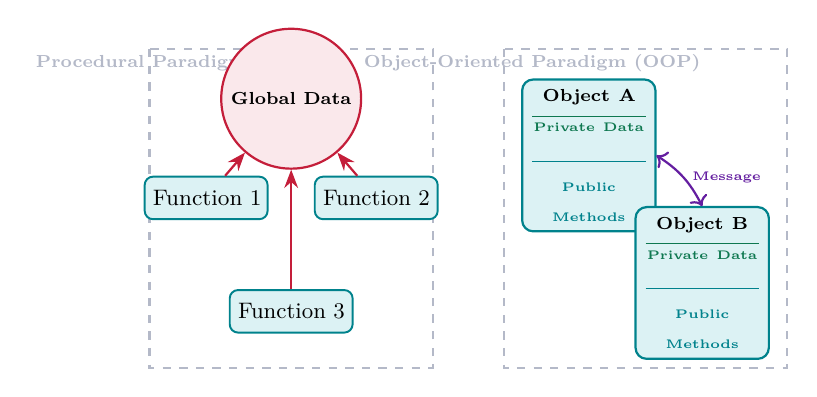
\begin{tikzpicture}[node distance=1.2cm, thick, scale=0.9, every node/.style={scale=0.9}]
  % Procedure-Oriented Model (Left side)
  \draw[dashed, color=mgframe] (-4, 2.5) rectangle (0, -2) node[pos=0.1, above, font=\scriptsize\bfseries\color{mydark}] {Procedural Paradigm (POP)};
  \node[circle, draw=myred, fill=hdrred, minimum size=1.0cm, font=\scriptsize\bfseries] (glob) at (-2, 1.8) {Global Data};
  \node[block, text width=1.5cm, minimum height=0.6cm] (f1) at (-3.2, 0.4) {Function 1};
  \node[block, text width=1.5cm, minimum height=0.6cm] (f2) at (-0.8, 0.4) {Function 2};
  \node[block, text width=1.5cm, minimum height=0.6cm] (f3) at (-2, -1.2) {Function 3};
  \draw[arrow, color=myred] (f1) -- (glob);
  \draw[arrow, color=myred] (f2) -- (glob);
  \draw[arrow, color=myred] (f3) -- (glob);

  % Object-Oriented Model (Right side)
  \draw[dashed, color=mgframe] (1, 2.5) rectangle (5, -2) node[pos=0.1, above, font=\scriptsize\bfseries\color{mydark}] {Object-Oriented Paradigm (OOP)};
  
  \node[draw=myteal, fill=hdrteal, rounded corners=4pt, text width=1.6cm, align=center, inner sep=4pt] (obj1) at (2.2, 1.0) {
    \scriptsize\bfseries Object A\\
    \color{mygreen}\rule{\linewidth}{0.4pt}
    \tiny Private Data\\
    \color{myteal}\rule{\linewidth}{0.4pt}
    \tiny Public Methods
  };

  \node[draw=myteal, fill=hdrteal, rounded corners=4pt, text width=1.6cm, align=center, inner sep=4pt] (obj2) at (3.8, -0.8) {
    \scriptsize\bfseries Object B\\
    \color{mygreen}\rule{\linewidth}{0.4pt}
    \tiny Private Data\\
    \color{myteal}\rule{\linewidth}{0.4pt}
    \tiny Public Methods
  };
  
  \draw[arrow, color=mypurple, <->, bend left=15] (obj1.east) to node[midway, right, font=\tiny\bfseries] {Message} (obj2.north);
\end{tikzpicture}
\end{tcolorbox}

% ===============================================================================
\section{Core Object-Oriented Programming Concepts}
% ===============================================================================

OOP seeks to model software systems in terms of real-world entities. Below are the foundational concepts of OOP:

\subsection{Objects and Classes}
\begin{tcolorbox}[defbox]
\textbf{Class:} A user-defined data type that acts as a blueprint, template, or prototype for creating objects. It defines the properties (data members) and actions (member functions) common to all objects of that class.
\par\vspace{3pt}
\textbf{Object:} A basic run-time entity of an object-oriented system that represents a real-world entity. It is an instance of a class, possessing its own state (data values) and behavior.
\end{tcolorbox}

\subsection{Data Encapsulation and Data Abstraction}
\begin{tcolorbox}[defbox]
\textbf{Data Encapsulation:} The mechanism of binding together code (member functions) and the data it manipulates (data members) into a single unit (class). It implements data hiding, keeping data safe from outside interference.
\par\vspace{3pt}
\textbf{Data Abstraction:} The act of representing essential features of a system without including the background details or implementation explanations. Users interact only with the interface, hiding complex execution.
\end{tcolorbox}

\subsection{Inheritance}
\begin{tcolorbox}[defbox]
\textbf{Inheritance:} The process by which objects of one class acquire the properties and behaviors of another class. It supports hierarchical classification and promotes \textbf{code reusability} by allowing new classes (derived classes) to extend existing ones (base classes).
\par\vspace{3pt}
\textbf{Base Class (Parent Class):} The class whose properties are inherited.
\par\vspace{3pt}
\textbf{Derived Class (Child Class):} The class that inherits from the base class.
\tcbset{colbacktitle=myteal, coltitle=white}
\end{tcolorbox}

\subsection{Polymorphism}
\begin{tcolorbox}[defbox]
\textbf{Polymorphism:} The ability of an interface to take multiple forms (from Greek, meaning "many forms"). It allows a single function name, operator symbol, or interface to behave differently depending on the context.
\end{tcolorbox}
There are two main classifications:
\begin{itemize}[leftmargin=*, itemsep=2pt]
  \item \textbf{Compile-Time (Static) Polymorphism:} Resolved at compile time (e.g., function overloading, operator overloading).
  \item \textbf{Run-Time (Dynamic) Polymorphism:} Resolved at runtime during execution (e.g., virtual functions, method overriding).
\end{itemize}

\subsection{Dynamic Binding and Message Passing}
\begin{tcolorbox}[defbox]
\textbf{Dynamic Binding:} The mechanism where the code associated with a given function call is not resolved until runtime. It is associated with inheritance and run-time polymorphism.
\par\vspace{3pt}
\textbf{Message Passing:} The communication process between objects. Objects interact by sending requests to execute methods of other objects, passing arguments and receiving results.
\end{tcolorbox}

% ===============================================================================
% MANDATORY QUICK REVISION PAGE
% ===============================================================================
\newpage
\begin{center}
  {\large\bfseries\color{myred} Quick Revision --- Module I}\\[3pt]
  {\small\color{mydark} Paradigm \& OOP Concepts $|$ OE-EC604C}
\end{center}
\noindent{\color{myred}\rule{\linewidth}{1.2pt}}
\vspace{4pt}

\begin{tcolorbox}[formulabox, title={\textbf{Key Concepts at a Glance}}]
\renewcommand{\arraystretch}{1.3}
\begin{tabularx}{\linewidth}{B{3.2cm} X}
Class Structure         & \texttt{class ClassName \{ private: // data public: // methods \};} \\[4pt]
The 4 Pillars of OOP    & \textbf{Encapsulation} (data hiding), \textbf{Abstraction} (interface separation), \textbf{Inheritance} (code reuse), \textbf{Polymorphism} (many forms). \\[4pt]
Access Modifiers        & \textbf{private}: Accessible only within class (default). \newline \textbf{public}: Accessible from anywhere. \newline \textbf{protected}: Accessible within class and child classes.
\end{tabularx}
\end{tcolorbox}

\begin{tcolorbox}[defbox, title={\textbf{One-Line Definitions}}]
\begin{itemize}[leftmargin=*, itemsep=2.5pt, topsep=0pt]
  \item \textbf{Paradigm:} A structured method or style of programming defining program organization.
  \item \textbf{Class:} A user-defined logical blueprint defining data and member functions.
  \item \textbf{Object:} A physical instance of a class representing a real-world entity.
  \item \textbf{Encapsulation:} Wrapping data and code together into a single unit (class) to prevent global access.
  \item \textbf{Data Hiding:} Restricting direct access to internal data members using access specifiers.
  \item \textbf{Abstraction:} Hiding background implementation details and exposing only the interface.
  \item \textbf{Inheritance:} The mechanism of deriving new classes from existing classes to achieve code reuse.
  \item \textbf{Polymorphism:} The capability of a function, operator, or object to act differently in different contexts.
  \item \textbf{Dynamic Binding:} Resolving method calls at runtime rather than compile time.
  \item \textbf{Message Passing:} Communication model where objects invoke member functions of other objects.
\end{itemize}
\end{tcolorbox}

\begin{tcolorbox}[exambox, title={\textbf{Frequently Asked / Viva Questions}}]
\begin{enumerate}[topsep=0pt, label=\textbf{Q\arabic*.}, itemsep=5pt]
  \item \Q{State the main limitation of Unstructured Programming.}
    Unstructured programming relies heavily on jump commands (like `goto`), making the control flow complex and highly difficult to trace, maintain, or debug.
  \item \Q{What is the core difference in how POP and OOP view data?}
    Procedure-Oriented Programming (POP) views data as passive elements manipulated by active procedures. OOP views data as critical assets tied securely to active functions.
  \item \Q{Define the difference between a Class and an Object.}
    A class is a logical template or blueprint (allocates no memory). An object is a physical instance of that template created in memory (allocates memory).
  \item \Q{Why does OOP offer better data security than POP?}
    OOP hides data members inside classes using the `private` access specifier, preventing outside functions from modifying the variables. POP global data is accessible to all.
  \item \Q{How does Encapsulation differ from Abstraction?}
    Encapsulation is the \textit{wrapping} or \textit{containment} of data (data hiding). Abstraction is the \textit{hiding of complexity} by showing only the external interface.
  \item \Q{What is the primary benefit of Inheritance?}
    Code reusability. It allows developer to extend base class properties without rewriting the code, reducing testing and development time.
  \item \Q{Explain the term "Polymorphism" with a real-world example.}
    A single instruction performs different actions based on target. E.g., the "+" symbol performs addition for numbers, but performs concatenation for strings.
  \item \Q{Define static binding vs. dynamic binding.}
    Static binding (early binding) resolves function calls at compile time. Dynamic binding (late binding) resolves function calls at runtime during execution.
  \item \Q{What is the role of access specifiers in C++?}
    Access specifiers (`private`, `public`, `protected`) control the visibility and accessibility of class members from outside classes.
  \item \Q{What is meant by the term "Message Passing"?}
    It is the process by which an object requests execution of a method belonging to another object, passing data parameters and receiving return values.
  \item \Q{Can you have an object without a class in C++?}
    No. In C++, every object must belong to a predefined class which defines its structure and member specifications.
  \item \Q{What is "Spaghetti Code" and in which paradigm does it commonly occur?}
    Spaghetti code is program code with highly convoluted control flow, usually caused by multiple jump statements (`goto`). It occurs in unstructured programming.
\end{enumerate}
\tcbset{colbacktitle=mypurple, coltitle=white}
\end{tcolorbox}

\begin{tcolorbox}[tikzbox, title={Comparison of POP and OOP Paradigms}]
\renewcommand{\arraystretch}{1.45}
\par\noindent
\begin{tabularx}{\linewidth}{|B{3.2cm}|Y|Y|}
\hline
\textbf{Parameter} & \textbf{\color{myteal}Procedure-Oriented (POP)} & \textbf{\color{mygreen}Object-Oriented (OOP)} \\
\hline
\textbf{Approach} & Top-down design methodology. & Bottom-up design methodology. \\
\hline
\textbf{Focus} & Focuses on the algorithm/process. & Focuses on the data assets. \\
\hline
\textbf{Data Access} & Functions share global data (unsafe). & Objects hide data using private scope (secure). \\
\hline
\textbf{Reusability} & Limited to function calls. & Achieved via class inheritance. \\
\hline
\textbf{Examples} & C, Pascal, Fortran. & C++, Java, Python, C\#. \\
\hline
\end{tabularx}
\end{tcolorbox}


% -- Module 2 -----------------------------------------------------------------
\modulestart{2}{C++ Streams, Namespaces \& Operators}

\section{C++ Streams, Namespaces \& Operators}
% ===============================================================================

C++ maintains backwards compatibility with C but introduces modern syntax and strict type checking to simplify development.

\subsection{Stream-Based Input/Output}
Unlike C which uses formatted functions like `printf` and `scanf`, C++ implements stream-based I/O. Streams are continuous sequences of bytes representing data flow.
\begin{itemize}[leftmargin=*, itemsep=3pt]
  \item \textbf{\texttt{cout}:} Standard output stream (connected to console), used with the stream insertion operator (\texttt{<<}).
  \item \textbf{\texttt{cin}:} Standard input stream (connected to keyboard), used with the stream extraction operator (\texttt{>>}).
  \item \textbf{Type Safety:} Operator overloading allows streams to automatically detect variables' data types (no format specifiers like \texttt{\%d} or \texttt{\%f} required).
\end{itemize}

\subsection{Namespaces}
\begin{tcolorbox}[defbox]
\textbf{Namespace:} A declarative region that provides a scope to the identifiers (names of types, functions, variables, etc.) inside it. Namespaces are used to organize code into logical groups and prevent name conflicts (clashing) in large projects.
\end{tcolorbox}
The C++ Standard Library is defined within a namespace named \textbf{\texttt{std}}. To use identifiers like `cout` or `cin`, we must specify their namespace:
\begin{align}
  &\text{using scope resolution: } \texttt{std::cout << "Hello";}\\
  &\text{using declaration: } \texttt{using std::cout; cout << "Hello";}\\
  &\text{using directive: } \texttt{using namespace std; cout << "Hello";}
\end{align}

\subsection{Scope Resolution Operator (\texttt{::})}
In C, if a local variable hides a global variable with the same name, there is no direct way to access the global variable. C++ introduces the scope resolution operator (\texttt{::}) to resolve scope conflicts.
\begin{tcolorbox}[formulabox, title={\textbf{Scope Resolution Syntax}}]
\begin{equation}
  \text{Global Variable Access: } \texttt{::variable\_name}
\end{equation}
It is also used for:
\begin{enumerate}[label=\alph*., leftmargin=1.5em, itemsep=1pt]
  \item Accessing static members of a class: \texttt{ClassName::static\_member}.
  \item Defining class member functions outside the class declaration.
  \item Resolving namespace paths: \texttt{NamespaceName::identifier}.
\end{enumerate}
\end{tcolorbox}

\begin{tcolorbox}[examplebox, title={Code Example: Global variable access via Scope Resolution}]
\begin{spacing}{1.0}
\begin{verbatim}
#include <iostream>
int x = 10; // Global variable
int main() {
    int x = 20; // Local variable hiding global x
    std::cout << "Local x = " << x << std::endl;      // Prints 20
    std::cout << "Global x = " << ::x << std::endl;    // Prints 10
    return 0;
}
\end{verbatim}
\end{spacing}
\end{tcolorbox}

\subsection{Variable Declaration and References}
\begin{itemize}[leftmargin=*, itemsep=3pt]
  \item \textbf{Declaration at Point of Use:} C requires variable declarations at the start of a block. C++ allows declaring variables anywhere in the code, immediately before their first use.
  \item \textbf{Reference Variables (Aliases):}
    \begin{tcolorbox}[defbox]
    \textbf{Reference Variable:} An alias or alternative name for an already existing variable. It shares the same memory space as the original variable. Modifying the reference modifies the original variable.
    \end{tcolorbox}
    \textbf{Declaration Syntax:}
    \begin{equation}
      \texttt{int x = 10; int \&y = x; // y is a reference to x}
    \end{equation}
    Reference variables must be initialized during declaration and cannot be re-bound to another variable.
\end{itemize}

% ===============================================================================
\section{Parameter Passing \& Functions}
% ===============================================================================

C++ extends function properties by introducing call-by-reference, inline compilation, and parameter defaults.

\subsection{Parameter Passing Mechanisms}
\begin{enumerate}[label=\textbf{\arabic*.}, leftmargin=*, itemsep=4pt]
  \item \textbf{Pass-by-Value:} A copy of the actual argument is passed to the function parameter. Changes inside the function do not affect the original variable.
  \item \textbf{Pass-by-Pointer:} The address of the argument is passed. The function dereferences the pointer to access/modify the original variable.
  \item \textbf{Pass-by-Reference:} The function parameter becomes an alias (reference) to the actual argument. No new memory is allocated, and the function directly manipulates the caller's variables.
\end{enumerate}

\begin{tcolorbox}[tikzbox, title={Memory Behavior of Parameter Passing}]
\centering
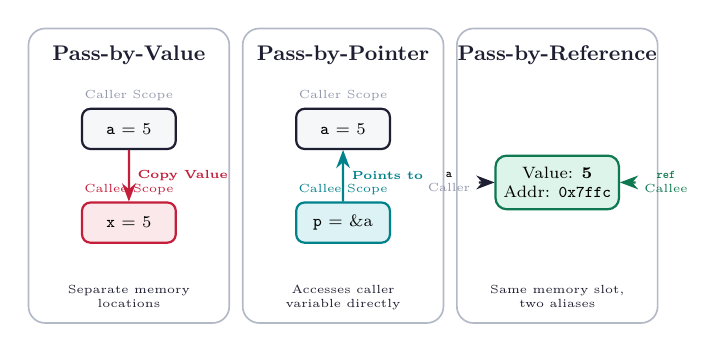
\begin{tikzpicture}[node distance=1.2cm, thick, scale=0.85, every node/.style={scale=0.85}]
  % Define styles locally
  \tikzset{
    varbox/.style={draw=mydark, fill=mygray, rounded corners=3pt, minimum width=1.4cm, minimum height=0.6cm, font=\scriptsize, align=center},
    card/.style={fill=white, draw=mgframe, rounded corners=6pt, line width=0.6pt}
  }

  % Pass-by-Value Card
  \draw[card] (-4.1, 2.2) rectangle (-1.1, -2.2);
  \node[font=\small\bfseries\color{mydark}] at (-2.6, 1.8) {Pass-by-Value};
  
  \node[font=\tiny\color{watermark}] at (-2.6, 1.2) {Caller Scope};
  \node[varbox] (val_caller) at (-2.6, 0.7) {\texttt{a} = 5};
  
  \node[font=\tiny\color{myred}] at (-2.6, -0.2) {Callee Scope};
  \node[varbox, draw=myred, fill=hdrred] (val_callee) at (-2.6, -0.7) {\texttt{x} = 5};
  
  \draw[arrow, color=myred] (val_caller) -- (val_callee) node[midway, right, font=\tiny\bfseries] {Copy Value};
  \node[below, font=\tiny\color{mydark}, align=center] at (-2.6, -1.5) {Separate memory\\locations};

  % Pass-by-Pointer Card
  \draw[card] (-0.9, 2.2) rectangle (2.1, -2.2);
  \node[font=\small\bfseries\color{mydark}] at (0.6, 1.8) {Pass-by-Pointer};
  
  \node[font=\tiny\color{watermark}] at (0.6, 1.2) {Caller Scope};
  \node[varbox] (ptr_caller) at (0.6, 0.7) {\texttt{a} = 5};
  
  \node[font=\tiny\color{myteal}] at (0.6, -0.2) {Callee Scope};
  \node[varbox, draw=myteal, fill=hdrteal] (ptr_callee) at (0.6, -0.7) {\texttt{p} = \&a};
  
  \draw[arrow, color=myteal] (ptr_callee) -- (ptr_caller) node[midway, right, font=\tiny\bfseries] {Points to};
  \node[below, font=\tiny\color{mydark}, align=center] at (0.6, -1.5) {Accesses caller\\variable directly};

  % Pass-by-Reference Card
  \draw[card] (2.3, 2.2) rectangle (5.3, -2.2);
  \node[font=\small\bfseries\color{mydark}] at (3.8, 1.8) {Pass-by-Reference};
  
  \node[draw=mygreen, fill=hdrgreen, rounded corners=4pt, minimum width=1.6cm, minimum height=0.8cm, font=\scriptsize, align=center] (ref_mem) at (3.8, -0.1) {Value: \textbf{5}\\Addr: \texttt{0x7ffc}};
  
  \node[left=0.2cm of ref_mem, align=center, font=\tiny] (ref_caller) {\textbf{\texttt{a}}\\\color{watermark}Caller};
  \node[right=0.2cm of ref_mem, align=center, font=\tiny\color{mygreen}] (ref_callee) {\textbf{\texttt{ref}}\\\color{mygreen}Callee};
  
  \draw[arrow] (ref_caller) -- (ref_mem.west);
  \draw[arrow, color=mygreen] (ref_callee) -- (ref_mem.east);
  
  \node[below, font=\tiny\color{mydark}, align=center] at (3.8, -1.5) {Same memory slot,\\two aliases};
\end{tikzpicture}
\end{tcolorbox}

\begin{tcolorbox}[examplebox, title={Code Example: Swapping variables using references}]
\begin{spacing}{1.0}
\begin{verbatim}
#include <iostream>
void swap(int &x, int &y) { // x and y are references to caller variables
    int temp = x;
    x = y;
    y = temp;
}
int main() {
    int a = 5, b = 10;
    swap(a, b); // Swaps values of a and b directly
    std::cout << "a = " << a << ", b = " << b; // Prints a = 10, b = 5
    return 0;
}
\end{verbatim}
\end{spacing}
\end{tcolorbox}

\subsection{Inline Functions}
Function calls introduce overhead: pushing arguments onto stack, saving registers, jumping to function address, restoring state on return. For small functions, the overhead can exceed the execution time of the function body.
\begin{tcolorbox}[defbox]
\textbf{Inline Function:} A function that is expanded in line at the point of call by the compiler instead of being invoked via standard function call stack jumps.
\end{tcolorbox}
\textbf{Syntax:}
\begin{equation}
  \texttt{inline int add(int a, int b) \{ return a + b; \}}
\end{equation}
\textbf{Key Rules and Compiler Discretion:}
The \texttt{inline} keyword is a \textbf{request}, not a command. The compiler can ignore it and compile the function normally if:
\begin{itemize}[leftmargin=*, itemsep=1pt, topsep=1pt]
  \item The function contains loops (\texttt{for}, \texttt{while}), switch statements, or goto.
  \item The function is recursive.
  \item The function contains static variables.
  \item The function returns a value but does not contain a return statement.
\end{itemize}

\subsection{Function Overloading}
Function overloading is a compile-time polymorphism feature allowing multiple functions to share the same name with different parameters.
\begin{tcolorbox}[defbox]
\textbf{Function Overloading:} The capability to declare multiple functions with the same name within the same scope, provided their signatures (parameter list) are unique.
\end{tcolorbox}
\textbf{Resolution Criteria:} The compiler distinguishes overloaded functions based on:
\begin{enumerate}[label=\textbf{\arabic*.}, leftmargin=1.5em, itemsep=1pt]
  \item \textbf{Number of parameters:} e.g., \texttt{void display(int)} vs \texttt{void display(int, int)}.
  \item \textbf{Type of parameters:} e.g., \texttt{void display(int)} vs \texttt{void display(double)}.
  \item \textbf{Order of parameters:} e.g., \texttt{void display(int, double)} vs \texttt{void display(double, int)}.
\end{enumerate}
\textbf{Note:} Functions cannot be overloaded based solely on their return types.

\subsection{Default Arguments}
Default arguments allow functions to assign a default value to a parameter if the caller does not provide an argument for it.
\textbf{Syntax:}
\begin{equation}
  \texttt{void printLine(char c = '*', int len = 40); // default values}
\end{equation}
\textbf{Critical Rule:}
Default arguments must be assigned from \textbf{right to left}. We cannot assign a default value to a parameter unless all parameters to its right also have default values.
\begin{align*}
  &\text{✅ Correct: } \texttt{void func(int a, int b = 10, int c = 20);}\\
  &\text{❌ Incorrect: } \texttt{void func(int a = 10, int b, int c = 20); // b lacks default}
\end{align*}

% ===============================================================================
% MANDATORY QUICK REVISION PAGE
% ===============================================================================
\newpage
\begin{center}
  {\large\bfseries\color{myred} Quick Revision --- Module II}\\[3pt]
  {\small\color{mydark} Moving from C to C++ $|$ OE-EC604C}
\end{center}
\noindent{\color{myred}\rule{\linewidth}{1.2pt}}
\vspace{4pt}

\begin{tcolorbox}[formulabox, title={\textbf{Key Formulas and Syntax}}]
\renewcommand{\arraystretch}{1.3}
\begin{tabularx}{\linewidth}{B{3.6cm} X}
Reference Variable      & \texttt{int x = 5; int \&ref = x; // ref shares memory with x} \\[4pt]
Inline Function         & \texttt{inline int square(int x) \{ return x * x; \}} \\[4pt]
Scope Resolution        & \texttt{::variable} \quad (accesses global variable hiding in local scope) \\[4pt]
Default Parameters      & \texttt{void value(int p, int n = 5, float r = 0.1); // right-to-left}
\end{tabularx}
\end{tcolorbox}

\begin{tcolorbox}[defbox, title={\textbf{One-Line Definitions}}]
\begin{itemize}[leftmargin=*, itemsep=2.5pt, topsep=0pt]
  \item \textbf{Reference Variable:} A constant pointer to variable that acts as an alternative name (alias) for that variable.
  \item \textbf{Namespace:} A scope region containing definitions to prevent name clashes in large programs.
  \item \textbf{Scope Resolution (::):} An operator used to access global variables or define class methods externally.
  \item \textbf{Inline Function:} A function that is compiled by replacing its calls directly with the function code.
  \item \textbf{Function Overloading:} Declaring multiple functions sharing the same name but unique parameters.
  \item \textbf{Default Argument:} A value assigned to a function parameter in its prototype used if argument is omitted.
  \item \textbf{Pass-by-Reference:} Passing parameters by sharing the caller's variable memory directly via references.
  \item \textbf{Type Safety:} Strict compile-time checks verifying variable types and function arguments matching.
\end{itemize}
\end{tcolorbox}

\begin{tcolorbox}[exambox, title={\textbf{Frequently Asked / Viva Questions}}]
\begin{enumerate}[topsep=0pt, label=\textbf{Q\arabic*.}, itemsep=5pt]
  \item \Q{Why does C++ input/output streams compile with greater type safety than C standard I/O?}
    C++ streams use overloaded insertion/extraction operators to automatically detect variable types, removing format specifier errors.
  \item \Q{Can we declare reference variables without initialization in C++?}
    No. A reference must be initialized to bind to a variable during declaration. E.g., `int \&ref;` causes a compile error.
  \item \Q{Can a reference variable be re-assigned to reference another variable later?}
    No. Once a reference variable is initialized to a target variable, it cannot be changed to reference any other variable.
  \item \Q{How does the scope resolution operator access global variables?}
    Adding the `::` prefix tells the compiler to search for the identifier in the global scope instead of the local stack block.
  \item \Q{What is the primary benefit of using inline functions?}
    It eliminates function call overhead (saving registers, jumping, stack frames), improving execution speed for small functions.
  \item \Q{Under what conditions will the C++ compiler ignore an inline request?}
    If the function is large, recursive, contains loops (`for`, `while`), switch/goto statements, or static variables.
  \item \Q{Can we overload a function based only on its return type?}
    No. The compiler resolves overloading by comparing parameter lists (number, type, order). Return types are ignored.
  \item \Q{State the mandatory rule for declaring default arguments in C++.}
    Default arguments must be added from right to left in the parameter list. No default argument can precede a non-default one.
  \item \Q{What is the difference between pass-by-pointer and pass-by-reference?}
    Pass-by-pointer passes a memory address (can be NULL, requires dereferencing). Pass-by-reference passes an alias (cannot be NULL, behaves like local variable).
  \item \Q{Explain the use of the `using namespace std;` statement.}
    It imports all identifiers from the standard library namespace (`std`) into global scope, removing the need to write `std::` prefixes.
  \item \Q{Why are inline functions preferred over preprocessor macros (\#define)?}
    Inline functions are compiled with full type-checking and follow scope and access rules, whereas macros are simple text replacements.
  \item \Q{What is a name collision/clash and how do namespaces solve it?}
    A name collision occurs when two libraries define classes or functions with identical names. Namespaces solve this by wrapping definitions in unique scope scopes.
\end{enumerate}
\tcbset{colbacktitle=mypurple, coltitle=white}
\end{tcolorbox}

\begin{tcolorbox}[tikzbox, title={Comparison of Parameter Passing Methods}]
\renewcommand{\arraystretch}{1.45}
\par\noindent
\begin{tabularx}{\linewidth}{|B{3.2cm}|Y|Y|Y|}
\hline
\textbf{Parameter} & \textbf{\color{myteal}Pass-by-Value} & \textbf{\color{myamber}Pass-by-Pointer} & \textbf{\color{mygreen}Pass-by-Reference} \\
\hline
\textbf{Memory Allocation} & Allocates new local storage for parameter copy. & Allocates storage for pointer address (4/8 bytes). & No new memory allocated. Shares caller's slot. \\
\hline
\textbf{Null Values} & Not applicable. & Pointer can be \texttt{nullptr}. & Reference cannot be null. \\
\hline
\textbf{Syntax} & Simple: \texttt{func(a)}. & Complex: \texttt{func(\&a)} and \texttt{*ptr}. & Simple: \texttt{func(a)} with parameter \texttt{\&ref}. \\
\hline
\textbf{Modifies Caller?} & No, operations are on copy. & Yes, via pointer dereferencing. & Yes, directly via alias. \\
\hline
\end{tabularx}
\end{tcolorbox}


% -- Module 3 -----------------------------------------------------------------
\modulestart{3}{Classes, Objects and Member Definitions}

\section{Classes, Objects and Member Definitions}
% ===============================================================================

In C++, classes serve as user-defined data types that bind data and operations together, forming the foundation of encapsulation.

\subsection{Specifying a Class and Access Specifiers}
A class is specified using the \texttt{class} keyword. Inside a class, variables (data members) and functions (member functions) are declared under three access levels:
\begin{itemize}[leftmargin=*, itemsep=3pt]
  \item \textbf{\texttt{private}:} Members declared private are accessible only inside member functions of the same class (default access level).
  \item \textbf{\texttt{public}:} Members are accessible from any part of the program where the class object is visible.
  \item \textbf{\texttt{protected}:} Members are accessible within the class itself and its derived (inherited) classes.
\end{itemize}

\subsection{Defining Class Member Functions}
Member functions can be defined in two ways:
\begin{enumerate}[label=\textbf{\arabic*.}, leftmargin=*, itemsep=4pt]
  \item \textbf{Inside the Class (Inline Definition):} Functions defined directly within the class declaration are implicitly treated as \texttt{inline} by the compiler.
  \item \textbf{Outside the Class (Scope Resolution):} Functions are declared inside the class and defined outside using the scope resolution operator (\texttt{::}).
\end{enumerate}

\begin{tcolorbox}[defbox, title={\textbf{Member Function Syntax Outside Class}}]
\begin{equation}
  \text{Return\_Type} \quad \text{Class\_Name}\texttt{::}\text{Function\_Name}(\text{Arguments}) \quad \{ \quad \text{Body} \quad \}
\end{equation}
\end{tcolorbox}

\begin{tcolorbox}[examplebox, title={Code Example: Inside vs. Outside class definitions}]
\begin{spacing}{1.0}
\begin{verbatim}
#include <iostream>
class Rectangle {
private:
    double length, width;
public:
    // Defined inside the class: treated as inline
    void setData(double l, double w) {
        length = l;
        width = w;
    }
    double getArea(); // Declared inside class, defined outside
};

// Defined outside using scope resolution
double Rectangle::getArea() {
    return length * width;
}
\end{verbatim}
\end{spacing}
\end{tcolorbox}

% ===============================================================================
\section{Static Data Members and Member Functions}
% ===============================================================================

Normally, every object has its own separate copy of all data members. However, static members allow sharing of data across all instances of a class.

\subsection{Static Data Members}
\begin{tcolorbox}[defbox]
\textbf{Static Data Member:} A variable declared with the \texttt{static} keyword inside a class. Only one copy of the static member is created for the entire class and is shared by all objects of that class, regardless of how many objects are instantiated.
\end{tcolorbox}
\textbf{Key Characteristics:}
\begin{itemize}[leftmargin=*, itemsep=2pt]
  \item \textbf{Lifetime:} It is initialized to 0 when the first object is created (unless initialized explicitly). It persists throughout the program execution.
  \item \textbf{Storage:} Allocated in the global static memory segment, not within the individual objects.
  \item \textbf{Definition Rule:} It must be defined and initialized outside the class block using the scope resolution operator.
\end{itemize}

\subsection{Static Member Functions}
A static member function can only access other static data members or static functions of the same class.
\textbf{Characteristics:}
\begin{itemize}[leftmargin=*, itemsep=2pt]
  \item Called using the class name: \texttt{ClassName::functionName()}. No object instance is required.
  \item Does not possess a \texttt{this} pointer (since it is not bound to a specific object instance).
\end{itemize}

\begin{tcolorbox}[examplebox, title={Code Example: Tracking Object Counts using Static Members}]
\begin{spacing}{1.0}
\begin{verbatim}
#include <iostream>
class Test {
private:
    int id;
    static int count; // Declaration of static member
public:
    Test() {
        count++;
        id = count;
    }
    void showId() {
        std::cout << "Object ID: " << id << std::endl;
    }
    static int getCount() { // Static member function
        return count; // Can only access static variables
    }
};

// Definition and initialization outside class (mandatory)
int Test::count = 0;

int main() {
    Test t1, t2;
    t1.showId(); // Object ID: 1
    t2.showId(); // Object ID: 2
    std::cout << "Total Objects: " << Test::getCount() << std::endl; // 2
    return 0;
}
\end{verbatim}
\end{spacing}
\end{tcolorbox}

% ===============================================================================
\section{Friend Functions and Friend Classes}
% ===============================================================================

To enforce data hiding, non-member functions are strictly blocked from accessing private class attributes. Friendships offer a controlled bypass.

\subsection{Friend Functions}
\begin{tcolorbox}[defbox]
\textbf{Friend Function:} A non-member function of a class that is granted permission to access the class's \texttt{private} and \texttt{protected} members. It is declared inside the class definition with the \texttt{friend} keyword.
\end{tcolorbox}

\textbf{Special Characteristics of Friend Functions:}
\begin{enumerate}[label=\textbf{\alph*.}, leftmargin=1.5em, itemsep=2pt]
  \item It is \textbf{not in the scope} of the class to which it has been declared a friend.
  \item It cannot be called using an object of that class (e.g., \texttt{obj.friendFunc()} is invalid). It is called like a normal global function: \texttt{friendFunc(obj)}.
  \item It usually takes class objects as arguments to process their private fields.
  \item It can be declared in either the \texttt{private} or \texttt{public} section of the class without altering its behavior.
\end{enumerate}

\begin{tcolorbox}[tikzbox, title={Friend Function Bridge Bypassing Class Access Restrictions}]
\centering
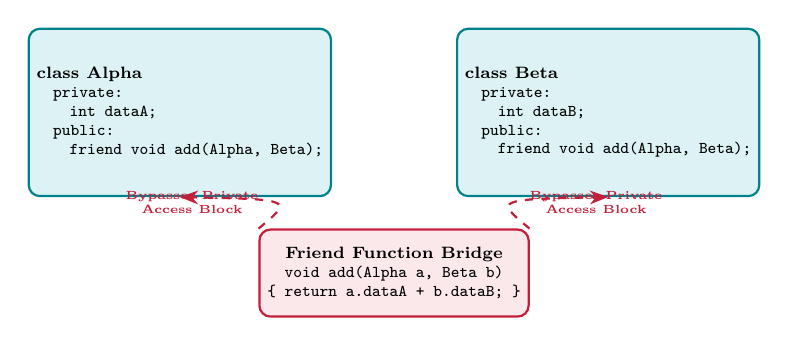
\begin{tikzpicture}[node distance=1.2cm, thick, scale=0.85, every node/.style={scale=0.85}]
  % Class Alpha box
  \node[rectangle, draw=myteal, fill=hdrteal, rounded corners=4pt, minimum width=3.4cm, minimum height=2.5cm, align=left, font=\scriptsize] (classA) at (-3.2, 0) {
    \textbf{class Alpha}\\
    \quad\texttt{private:}\\
    \quad\quad\texttt{int dataA;}\\
    \quad\texttt{public:}\\
    \quad\quad\texttt{friend void add(Alpha, Beta);}
  };

  % Class Beta box
  \node[rectangle, draw=myteal, fill=hdrteal, rounded corners=4pt, minimum width=3.4cm, minimum height=2.5cm, align=left, font=\scriptsize] (classB) at (3.2, 0) {
    \textbf{class Beta}\\
    \quad\texttt{private:}\\
    \quad\quad\texttt{int dataB;}\\
    \quad\texttt{public:}\\
    \quad\quad\texttt{friend void add(Alpha, Beta);}
  };

  % Friend function box (Bridge)
  \node[rectangle, draw=myred, fill=hdrred, rounded corners=4pt, minimum width=4.0cm, minimum height=1.3cm, align=center, font=\scriptsize] (friendFunc) at (0, -2.4) {
    \textbf{Friend Function Bridge}\\
    \texttt{void add(Alpha a, Beta b)}\\
    \texttt{\{ return a.dataA + b.dataB; \}}
  };

  % Path/Bridge
  \draw[arrow, color=myred, dashed, line width=0.8pt] (friendFunc.north west) .. controls (-1.5, -1.3) .. (classA.south) 
    node[midway, left=0.1cm, font=\tiny\bfseries, align=center] {Bypasses Private\\Access Block};
  \draw[arrow, color=myred, dashed, line width=0.8pt] (friendFunc.north east) .. controls (1.5, -1.3) .. (classB.south) 
    node[midway, right=0.1cm, font=\tiny\bfseries, align=center] {Bypasses Private\\Access Block};
\end{tikzpicture}
\end{tcolorbox}

\begin{tcolorbox}[examplebox, title={Code Example: Friend Function accessing private variables of two classes}]
\begin{spacing}{1.0}
\begin{verbatim}
#include <iostream>
class Beta; // Forward declaration required for Alpha's friend prototype

class Alpha {
private:
    int valA;
public:
    Alpha(int v) : valA(v) {}
    friend int add(Alpha, Beta); // Declare friend function
};

class Beta {
private:
    int valB;
public:
    Beta(int v) : valB(v) {}
    friend int add(Alpha, Beta); // Declare same function as friend
};

// Friend function definition (no 'friend' keyword or scope resolution here)
int add(Alpha a, Beta b) {
    return a.valA + b.valB; // Directly accessing private members
}

int main() {
    Alpha a(15);
    Beta b(25);
    std::cout << "Sum = " << add(a, b); // Outputs: Sum = 40
    return 0;
}
\end{verbatim}
\end{spacing}
\tcbset{colbacktitle=myamber, coltitle=white}
\end{tcolorbox}

\subsection{Friend Classes}
A class can also be declared as a friend of another class. If \texttt{class B} is declared as a \texttt{friend} inside \texttt{class A}, then \textbf{all} member functions of \texttt{class B} gain access to the private and protected data members of \texttt{class A}.
\begin{equation}
  \texttt{class A \{ friend class B; \}; // Class B is a friend of Class A}
\end{equation}

% ===============================================================================
\section{Object Memory and Dynamic Allocation}
% ===============================================================================

To write efficient code, engineers must understand how objects occupy physical memory and how dynamic memory operators allocate resources on the heap.

\subsection{Memory Considerations for Objects}
When a class is declared, no memory is allocated. Memory is only allocated when objects of that class are instantiated.
\begin{itemize}[leftmargin=*, itemsep=3pt]
  \item \textbf{Data Members:} Each object receives its own independent memory allocation for non-static data members (to hold distinct object states).
  \item \textbf{Member Functions:} Member functions are allocated only once in the \textbf{Code Segment} when the class is loaded. All objects of the class share the exact same memory space for functions. This prevents code redundancy.
\end{itemize}

\begin{tcolorbox}[tikzbox, title={Object Memory Allocation Layout in RAM}]
\centering
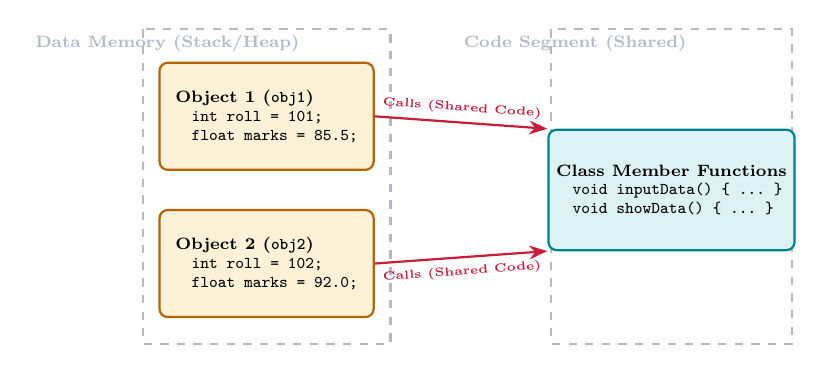
\begin{tikzpicture}[node distance=1.2cm, thick, scale=0.85, every node/.style={scale=0.85}]
  % Stack/Heap (Separate Data Memory)
  \draw[dashed, color=mgframe] (-4.5, 2.2) rectangle (-0.8, -2.5) node[pos=0.1, above, font=\scriptsize\bfseries] {Data Memory (Stack/Heap)};
  
  \node[rectangle, draw=myamber, fill=hdramber, rounded corners=3pt, minimum width=3.2cm, minimum height=1.6cm, align=left, font=\scriptsize] (obj1) at (-2.65, 0.9) {
    \textbf{Object 1 (\texttt{obj1})}\\
    \quad\texttt{int roll = 101;}\\
    \quad\texttt{float marks = 85.5;}
  };
  
  \node[rectangle, draw=myamber, fill=hdramber, rounded corners=3pt, minimum width=3.2cm, minimum height=1.6cm, align=left, font=\scriptsize] (obj2) at (-2.65, -1.3) {
    \textbf{Object 2 (\texttt{obj2})}\\
    \quad\texttt{int roll = 102;}\\
    \quad\texttt{float marks = 92.0;}
  };

  % Code Segment (Shared member functions)
  \draw[dashed, color=mgframe] (1.6, 2.2) rectangle (5.2, -2.5) node[pos=0.1, above, font=\scriptsize\bfseries] {Code Segment (Shared)};
  
  \node[rectangle, draw=myteal, fill=hdrteal, rounded corners=3pt, minimum width=3.2cm, minimum height=1.8cm, align=left, font=\scriptsize] (code) at (3.4, -0.2) {
    \textbf{Class Member Functions}\\
    \quad\texttt{void inputData() \{ ... \}}\\
    \quad\texttt{void showData() \{ ... \}}
  };

  % Arrows representing function invocation
  \draw[arrow, color=myred] (obj1.east) -- (code.north west) node[midway, above, sloped, font=\tiny\bfseries] {Calls (Shared Code)};
  \draw[arrow, color=myred] (obj2.east) -- (code.south west) node[midway, below, sloped, font=\tiny\bfseries] {Calls (Shared Code)};
\end{tikzpicture}
\tcbset{colbacktitle=mgframe, coltitle=mydark}
\end{tcolorbox}

\subsection{Dynamic Memory Management: \texorpdfstring{\texttt{new}}{new} and \texorpdfstring{\texttt{delete}}{delete}}
In addition to C's run-time allocation functions (\texttt{malloc}/\texttt{free}), C++ introduces type-safe operators \texttt{new} and \texttt{delete} which operate directly on the Heap memory.

\begin{tcolorbox}[formulabox, title={\textbf{Dynamic Memory Syntax}}]
\begin{align}
  &\text{Allocate Single Variable: } && \texttt{pointer\_var = new data\_type;} \\
  &\text{Allocate Array of Elements: } && \texttt{pointer\_var = new data\_type[size];} \\
  &\text{Deallocate Single Variable: } && \texttt{delete pointer\_var;} \\
  &\text{Deallocate Array: } && \texttt{delete [] pointer\_var;}
\end{align}
\end{tcolorbox}

\textbf{Advantages of \texttt{new}/\texttt{delete} over \texttt{malloc}/\texttt{free}:}
\begin{enumerate}[label=\textbf{\arabic*.}, leftmargin=*, itemsep=2pt]
  \item \textbf{Constructor Calling:} \texttt{new} automatically calls the object's constructor; \texttt{malloc} only allocates raw bytes.
  \item \textbf{Destructor Calling:} \texttt{delete} automatically calls the destructor before freeing memory; \texttt{free} does not.
  \item \textbf{Type Safety:} \texttt{new} returns the exact pointer type (no explicit typecasting needed); \texttt{malloc} returns a \texttt{void*}.
  \item \textbf{Safety:} \texttt{new} throws a \texttt{std::bad\_alloc} exception if allocation fails; \texttt{malloc} returns \texttt{NULL}.
\end{enumerate}

\begin{tcolorbox}[examplebox, title={Code Example: Dynamic allocation of variable and array}]
\begin{spacing}{1.0}
\begin{verbatim}
#include <iostream>
int main() {
    // Dynamic single variable allocation
    int *pInt = new int(42); // Allocates int and initializes to 42
    std::cout << "Value: " << *pInt << std::endl;
    delete pInt; // Free memory

    // Dynamic array allocation
    int size = 5;
    int *arr = new int[size]; // Allocates array of 5 integers
    for (int i = 0; i < size; i++) {
        arr[i] = (i + 1) * 10;
        std::cout << arr[i] << " ";
    }
    std::cout << std::endl;
    
    delete[] arr; // Free array memory (note the square brackets)
    return 0;
}
\end{verbatim}
\end{spacing}
\tcbset{colbacktitle=myamber, coltitle=white}
\end{tcolorbox}

% ===============================================================================
% MANDATORY QUICK REVISION PAGE
% ===============================================================================
\newpage
\begin{center}
  {\large\bfseries\color{myred} Quick Revision --- Module III}\\[3pt]
  {\small\color{mydark} Objects and Classes $|$ OE-EC604C}
\end{center}
\noindent{\color{myred}\rule{\linewidth}{1.2pt}}
\vspace{4pt}

\begin{tcolorbox}[formulabox, title={\textbf{Key Syntax and Configurations}}]
\renewcommand{\arraystretch}{1.3}
\begin{tabularx}{\linewidth}{B{3.8cm} X}
Class Declaration        & \texttt{class MyClass \{ private: int x; public: void func(); \};} \\[4pt]
External Definition      & \texttt{void MyClass::func() \{ /* code */ \}} \\[4pt]
Static Definition        & \texttt{int MyClass::staticVar = 0; // Out-of-class definition} \\[4pt]
Friend Declaration       & \texttt{friend void myFriend(MyClass \&obj); // Inside class} \\[4pt]
Dynamic Single           & \texttt{int *ptr = new int(10); \quad delete ptr;} \\[4pt]
Dynamic Array            & \texttt{int *arr = new int[5]; \quad delete [] arr;}
\end{tabularx}
\end{tcolorbox}

\begin{tcolorbox}[defbox, title={\textbf{One-Line Definitions}}]
\begin{itemize}[leftmargin=*, itemsep=2.5pt, topsep=0pt]
  \item \textbf{Class:} A user-defined data type that binds data and functions together into a single unit.
  \item \textbf{Object:} An instance of a class that represents a real-world entity and occupies memory.
  \item \textbf{Access Specifiers:} Keywords (\texttt{private}, \texttt{public}, \texttt{protected}) that define the accessibility of class members.
  \item \textbf{Static Data Member:} A class variable shared by all class objects, residing in global static memory.
  \item \textbf{Static Member Function:} A function that can only access static members and is called without an object.
  \item \textbf{Friend Function:} A non-member function declared inside a class that can access its private and protected members.
  \item \textbf{Friend Class:} A class whose member functions can all access the private and protected members of another class.
  \item \textbf{new Operator:} A C++ operator used to dynamically allocate memory on the heap and run constructors.
  \item \textbf{delete Operator:} A C++ operator used to release dynamically allocated heap memory and run destructors.
\end{itemize}
\end{tcolorbox}

\begin{tcolorbox}[exambox, title={\textbf{Frequently Asked / Viva Questions}}]
\begin{enumerate}[topsep=0pt, label=\textbf{Q\arabic*.}, itemsep=5pt]
  \item \Q{What is the default access specifier for class members in C++?}
    The default access specifier is `private`. If no access specifier is mentioned, members are treated as private.
  \item \Q{Why do member functions defined inside the class run faster than those defined outside?}
    Member functions defined inside the class are implicitly treated as `inline`, meaning the compiler attempts to substitute the call site with the function code, avoiding call overhead.
  \item \Q{Why must static data members be defined outside the class scope?}
    The class declaration only defines the type, it does not allocate memory. Defining it outside allocates physical storage in global memory.
  \item \Q{Can a static member function access non-static variables of the class?}
    No. A static function is not bound to any object instance, so it lacks a `this` pointer and cannot determine which object's non-static variable to access.
  \item \Q{Explain why a friend function cannot be called using the object dot (.) operator.}
    A friend function is not a member of the class. It is a normal global function with special access rights, so calling it with `obj.` causes a compile error.
  \item \Q{Does declaring a friend function inside a class violate encapsulation?}
    Theoretically yes, as it bypasses private access blocks. However, it is controlled by the class designer and is useful for operations like operator overloading.
  \item \Q{What is the memory size of an empty class object in C++?}
    It is 1 byte. The compiler allocates 1 byte to ensure that two different object instances of the empty class have unique memory addresses.
  \item \Q{What happens if you use `delete` instead of `delete []` to free a dynamically allocated array?}
    It results in undefined behavior. Typically, the compiler will only call the destructor for the first element in the array and may fail to release the entire block of memory.
  \item \Q{What is the difference between class and struct in C++?}
    In a `struct`, members are `public` by default, whereas in a `class`, members are `private` by default.
  \item \Q{Can we declare a constructor static in C++?}
    No. Constructors are called to initialize specific object instances. A static function has no instance binding, making a static constructor logically impossible.
  \item \Q{Does `new` return a void pointer like `malloc`?}
    No. The `new` operator is type-safe and returns a typed pointer to the allocated memory, eliminating the need for casting.
  \item \Q{Can we overload a friend function?}
    Yes, a friend function is a regular function and can be overloaded like any other non-member function.
\end{enumerate}
\tcbset{colbacktitle=mypurple, coltitle=white}
\end{tcolorbox}

\begin{tcolorbox}[tikzbox, title={Comparison: C++ dynamic operators vs. C memory functions}]
\renewcommand{\arraystretch}{1.45}
\par\noindent
\begin{tabularx}{\linewidth}{|B{3.2cm}|Y|Y|}
\hline
\textbf{Feature} & \textbf{\color{myteal}new / delete (C++)} & \textbf{\color{myamber}malloc / free (C)} \\
\hline
\textbf{Type Safety} & Type-safe; returns exact type pointer. & Returns \texttt{void*}; requires explicit typecasting. \\
\hline
\textbf{Constructors} & Calls constructors automatically for classes. & Does not trigger constructors (allocates raw bytes). \\
\hline
\textbf{Destructors} & Calls destructors automatically. & Does not trigger destructors. \\
\hline
\textbf{Failure Behavior} & Throws \texttt{std::bad\_alloc} exception. & Returns \texttt{NULL}. \\
\hline
\textbf{Buffer Size} & Automatically calculated by compiler. & Must be explicitly calculated in bytes using \texttt{sizeof}. \\
\hline
\end{tabularx}
\end{tcolorbox}


% -- Module 4 -----------------------------------------------------------------
\modulestart{4}{Fundamentals of Constructors}

\section{Fundamentals of Constructors}
% ===============================================================================

Constructors are special member functions of a class designed specifically to initialize objects during instantiation.

\subsection{Rules and Characteristics}
A constructor must follow strict compiler rules:
\begin{itemize}[leftmargin=*, itemsep=3pt]
  \item \textbf{Naming:} It must have the exact same name as the class.
  \item \textbf{Return Type:} It does not have any return type, not even \texttt{void}.
  \item \textbf{Execution:} It is automatically invoked by the system when an object of the class is created.
  \item \textbf{Implicit/Explicit Invocation:} 
    \begin{align}
      &\text{Implicit call: } \texttt{Complex c1(5, 10);} \\
      &\text{Explicit call: } \texttt{Complex c1 = Complex(5, 10);}
    \end{align}
  \item \textbf{Restrictions:} It cannot be declared \texttt{virtual}, \texttt{static}, or \texttt{const}.
\end{itemize}

\subsection{Types of Constructors}
\begin{enumerate}[label=\textbf{\arabic*.}, leftmargin=*, itemsep=4pt]
  \item \textbf{Default Constructor:} A constructor that accepts no arguments. If no constructor is written, the compiler automatically generates a default constructor.
  \item \textbf{Parameterized Constructor:} A constructor that accepts arguments, allowing objects to be initialized with custom values at creation time.
  \item \textbf{Copy Constructor:} Used to initialize an object using values of another pre-existing object of the same class.
  \item \textbf{Dynamic Constructor:} A constructor that uses the \texttt{new} operator to allocate dynamic heap memory for members during object creation.
\end{enumerate}

% ===============================================================================
\section{Deep Copying and Shallow Copying}
% ===============================================================================

Copy operations in C++ can lead to critical memory bugs if pointers are involved.

\subsection{Shallow Copy vs. Deep Copy}
\begin{itemize}[leftmargin=*, itemsep=3pt]
  \item \textbf{Shallow Copy:} The compiler copies member variables bit-by-bit. If a class contains pointers to heap memory, only the address is copied. As a result, both the original and copied objects point to the same memory block.
    \begin{tcolorbox}[defbox]
    \textbf{Shallow Copy Risk:} When either object is destroyed, its destructor runs and frees the shared heap memory. The remaining object is left with a dangling pointer, and attempting to delete it results in a double-free crash.
    \end{tcolorbox}
  \item \textbf{Deep Copy:} A user-defined copy constructor allocates a separate block of heap memory and copies the actual values from the source buffer. This isolates the memory blocks.
\end{itemize}

\begin{tcolorbox}[tikzbox, title={Memory Block Mappings: Shallow Copy vs. Deep Copy}]
\centering
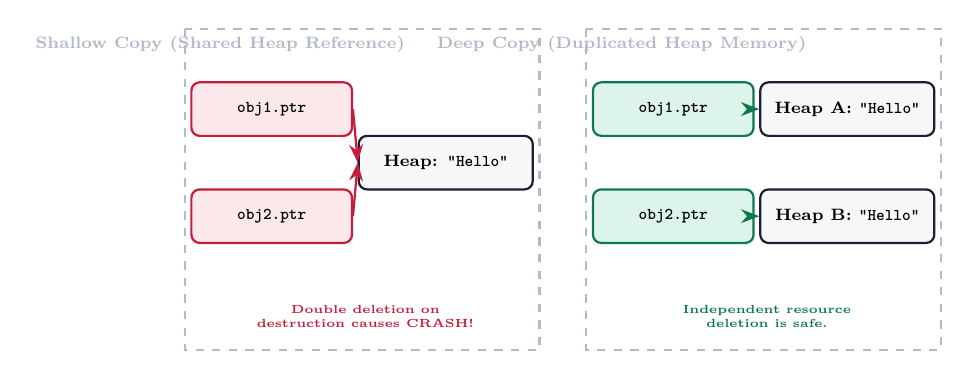
\begin{tikzpicture}[node distance=1.2cm, thick, scale=0.85, every node/.style={scale=0.85}]
  % --- SHALLOW COPY BLOCK ---
  \draw[dashed, color=mgframe] (-4.5, 2.2) rectangle (0.8, -2.6) node[pos=0.1, above, font=\scriptsize\bfseries] {Shallow Copy (Shared Heap Reference)};
  
  \node[draw=myred, fill=hdrred, rounded corners=3pt, minimum width=2.4cm, minimum height=0.8cm, font=\scriptsize\bfseries] (s_obj1) at (-3.2, 1.0) {\texttt{obj1.ptr}};
  \node[draw=myred, fill=hdrred, rounded corners=3pt, minimum width=2.4cm, minimum height=0.8cm, font=\scriptsize\bfseries] (s_obj2) at (-3.2, -0.6) {\texttt{obj2.ptr}};
  
  \node[draw=mydark, fill=mygray, rounded corners=3pt, minimum width=2.6cm, minimum height=0.8cm, font=\scriptsize\bfseries] (s_heap) at (-0.6, 0.2) {Heap: \texttt{"Hello"}};
  
  \draw[arrow, color=myred] (s_obj1.east) -- (s_heap.west);
  \draw[arrow, color=myred] (s_obj2.east) -- (s_heap.west);
  \node[below, font=\tiny\bfseries\color{myred}, align=center] at (-1.8, -1.8) {Double deletion on\\destruction causes CRASH!};

  % --- DEEP COPY BLOCK ---
  \draw[dashed, color=mgframe] (1.5, 2.2) rectangle (6.8, -2.6) node[pos=0.1, above, font=\scriptsize\bfseries] {Deep Copy (Duplicated Heap Memory)};
  
  \node[draw=mygreen, fill=hdrgreen, rounded corners=3pt, minimum width=2.4cm, minimum height=0.8cm, font=\scriptsize\bfseries] (d_obj1) at (2.8, 1.0) {\texttt{obj1.ptr}};
  \node[draw=mygreen, fill=hdrgreen, rounded corners=3pt, minimum width=2.4cm, minimum height=0.8cm, font=\scriptsize\bfseries] (d_obj2) at (2.8, -0.6) {\texttt{obj2.ptr}};
  
  \node[draw=mydark, fill=mygray, rounded corners=3pt, minimum width=2.6cm, minimum height=0.8cm, font=\scriptsize\bfseries] (d_heap1) at (5.4, 1.0) {Heap A: \texttt{"Hello"}};
  \node[draw=mydark, fill=mygray, rounded corners=3pt, minimum width=2.6cm, minimum height=0.8cm, font=\scriptsize\bfseries] (d_heap2) at (5.4, -0.6) {Heap B: \texttt{"Hello"}};
  
  \draw[arrow, color=mygreen] (d_obj1.east) -- (d_heap1.west);
  \draw[arrow, color=mygreen] (d_obj2.east) -- (d_heap2.west);
  \node[below, font=\tiny\bfseries\color{mygreen}, align=center] at (4.2, -1.8) {Independent resource\\deletion is safe.};
\end{tikzpicture}
\tcbset{colbacktitle=mgframe, coltitle=mydark}
\end{tcolorbox}

\begin{tcolorbox}[examplebox, title={Code Example: String copy constructor (Deep Copy)}]
\begin{spacing}{1.0}
\begin{verbatim}
#include <iostream>
#include <cstring>
class String {
private:
    char *str;
    int len;
public:
    String(const char *s) {
        len = strlen(s);
        str = new char[len + 1];
        strcpy(str, s);
    }
    // Deep Copy Constructor
    String(const String &source) {
        len = source.len;
        str = new char[len + 1]; // Allocate separate heap memory
        strcpy(str, source.str); // Copy actual data contents
        std::cout << "Copy Constructor Called (Deep Copy)" << std::endl;
    }
    ~String() {
        delete[] str; // Free local pointer safely
    }
    void display() { std::cout << str << std::endl; }
};
\end{verbatim}
\end{spacing}
\tcbset{colbacktitle=myamber, coltitle=white}
\end{tcolorbox}

% ===============================================================================
\section{Constructor Overloading \& Destructors}
% ===============================================================================

C++ allows multiple constructors in a class, selecting the correct one based on arguments. It also ensures proper cleanup when objects go out of scope.

\subsection{Constructor Overloading and Default Arguments}
Classes can have multiple constructors with different parameter signatures. They can also contain default arguments.
\begin{align*}
  &\text{Constructor 1 (Default): } && \texttt{Complex() \{ real = imag = 0; \}} \\
  &\text{Constructor 2 (Parameterized): } && \texttt{Complex(double r, double i = 0) \{ real = r; imag = i; \}}
\end{align*}

\subsection{Destructors}
\begin{tcolorbox}[defbox]
\textbf{Destructor:} A special member function of a class that is called automatically when an object goes out of scope or is explicitly deleted. Its purpose is to release resource allocations (like heap memory, open file handlers, socket connections).
\end{tcolorbox}

\textbf{Key Destructor Rules:}
\begin{itemize}[leftmargin=*, itemsep=2pt]
  \item Naming: Same name as class, prefixed with a tilde symbol (\texttt{\textasciitilde}).
  \item Arguments: Cannot take any parameters or return values. Overloading is not possible.
  \item Execution Order: Objects are destroyed in the \textbf{reverse order} of their creation (Last In, First Out).
\end{itemize}

\begin{tcolorbox}[examplebox, title={Code Example: Tracing Constructor and Destructor Executions}]
\begin{spacing}{1.0}
\begin{verbatim}
#include <iostream>
class Trace {
private:
    int id;
public:
    Trace(int val) : id(val) {
        std::cout << "Constructor called for " << id << std::endl;
    }
    ~Trace() {
        std::cout << "Destructor called for " << id << std::endl;
    }
};

void runLocal() {
    std::cout << "--- Enter local scope ---" << std::endl;
    Trace localObj(2);
    std::cout << "--- Exit local scope ---" << std::endl;
}

int main() {
    std::cout << "--- Main Start ---" << std::endl;
    Trace globalObj(1);
    runLocal();
    std::cout << "--- Main End ---" << std::endl;
    return 0;
}
\end{verbatim}
\end{spacing}
\tcbset{colbacktitle=myamber, coltitle=white}
\end{tcolorbox}
The code above outputs:
\begin{verbatim}
--- Main Start ---
Constructor called for 1
--- Enter local scope ---
Constructor called for 2
--- Exit local scope ---
Destructor called for 2
--- Main End ---
Destructor called for 1
\end{verbatim}

% ===============================================================================
% MANDATORY QUICK REVISION PAGE
% ===============================================================================
\newpage
\begin{center}
  {\large\bfseries\color{myred} Quick Revision --- Module IV}\\[3pt]
  {\small\color{mydark} Constructors and Destructors $|$ OE-EC604C}
\end{center}
\noindent{\color{myred}\rule{\linewidth}{1.2pt}}
\vspace{4pt}

\begin{tcolorbox}[formulabox, title={\textbf{Key Constructor Syntax}}]
\renewcommand{\arraystretch}{1.3}
\begin{tabularx}{\linewidth}{B{3.8cm} X}
Default Constructor      & \texttt{MyClass() \{ x = 0; \}} \\[4pt]
Parameterized            & \texttt{MyClass(int val) : x(val) \{ \} // uses initializer list} \\[4pt]
Copy Constructor         & \texttt{MyClass(const MyClass \&src) \{ x = src.x; \} // reference is mandatory} \\[4pt]
Destructor               & \texttt{\textasciitilde MyClass() \{ /* release heap memory / close files */ \}}
\end{tabularx}
\end{tcolorbox}

\begin{tcolorbox}[defbox, title={\textbf{One-Line Definitions}}]
\begin{itemize}[leftmargin=*, itemsep=2.5pt, topsep=0pt]
  \item \textbf{Constructor:} A special member function with the class name that initializes objects upon instantiation.
  \item \textbf{Default Constructor:} A constructor that takes no parameters (either empty or with all arguments defaulted).
  \item \textbf{Copy Constructor:} A constructor used to create an object as a clone of an existing object of the same class.
  \item \textbf{Dynamic Constructor:} A constructor that allocates heap memory dynamically during object initialization.
  \item \textbf{Destructor:} A special member function prefixed with \texttt{\textasciitilde} that deallocates resources when an object is destroyed.
  \item \textbf{Shallow Copy:} A member-by-member copy of an object, copying pointer addresses rather than the target data.
  \item \textbf{Deep Copy:} A copy operation that duplicates the heap resources pointed to by an object, creating an independent clone.
  \item \textbf{Initializer List:} A comma-separated list prefixing a constructor body used to initialize data members directly.
  \item \textbf{Double Deletion:} A crash state occurring when two objects point to the same heap block and both attempt to delete it.
\end{itemize}
\end{tcolorbox}

\begin{tcolorbox}[exambox, title={\textbf{Frequently Asked / Viva Questions}}]
\begin{enumerate}[topsep=0pt, label=\textbf{Q\arabic*.}, itemsep=5pt]
  \item \Q{Why is it mandatory to pass the argument by reference in a copy constructor?}
    If passed by value, the function call itself would invoke the copy constructor to clone the parameter, causing infinite recursion until the stack overflows. E.g., `MyClass(MyClass source)` is incorrect.
  \item \Q{Can a class have more than one destructor?}
    No. Destructors cannot accept arguments, which means they cannot be overloaded. Every class has exactly one destructor.
  \item \Q{Under what conditions does the C++ compiler write a default copy constructor for you?}
    If a class does not define any copy constructor, the compiler automatically generates a default copy constructor, which performs a shallow copy.
  \item \Q{Explain the order of execution of constructors and destructors in hybrid structures.}
    Constructors are invoked in the order of inheritance (base classes first, then derived classes). Destructors run in the exact reverse order.
  \item \Q{Is it possible to declare a private constructor in C++?}
    Yes. A private constructor prevents objects from being created outside the class scope. This pattern is commonly used in the Singleton Design Pattern.
  \item \Q{What is the difference between copy constructor and assignment operator (\texttt{=})?}
    The copy constructor initializes a newly created object using a source object (e.g., `MyClass a = b;`). The assignment operator copies values to an already existing object (e.g., `a = b;`).
  \item \Q{Does a destructor release the memory of the object itself?}
    No. A destructor only frees auxiliary resources allocated \textit{inside} the object (e.g., heap pointers, file descriptors). The memory for the object structure itself is freed by the stack or heap manager.
  \item \Q{Why can't we declare a constructor as `virtual`?}
    Virtual functions rely on the V-Table (virtual table) pointer inside an object. During construction, the object is not fully formed, and the V-Ptr is not yet initialized. Thus, constructors cannot be virtual.
  \item \Q{What is the purpose of declaring copy constructor arguments as `const`?}
    Declaring the argument as `const` (e.g., `const MyClass \&obj`) prevents the copy constructor from accidentally modifying the source object.
  \item \Q{What is a member initializer list and when is it mandatory?}
    It is a constructor mechanism used to initialize members directly. It is mandatory for: (1) initializing reference variables, (2) initializing `const` members, and (3) calling parameterized base class constructors.
  \item \Q{Can we call a constructor explicitly like a normal function?}
    Yes, we can call it explicitly (e.g., `Complex c = Complex(1.0, 2.0);`), which creates a temporary object that is then copied or moved.
  \item \Q{What happens if an exception is thrown inside a constructor?}
    If an exception is thrown in a constructor, the object is considered only partially constructed, and its destructor will not run. This can lead to memory leaks unless resources are managed via smart pointers.
\end{enumerate}
\tcbset{colbacktitle=mypurple, coltitle=white}
\end{tcolorbox}

\begin{tcolorbox}[tikzbox, title={Comparison: Shallow Copy vs. Deep Copy}]
\renewcommand{\arraystretch}{1.45}
\par\noindent
\begin{tabularx}{\linewidth}{|B{3.2cm}|Y|Y|}
\hline
\textbf{Feature} & \textbf{\color{myred}Shallow Copy} & \textbf{\color{mygreen}Deep Copy} \\
\hline
\textbf{Heap Memory} & Shares the existing heap memory between objects. & Allocates new, independent memory blocks on the heap. \\
\hline
\textbf{Pointer Safety} & Pointer address is copied. Vulnerable to dangling pointers. & Pointers point to separate blocks. Safe from cross-corruption. \\
\hline
\textbf{Crash Risk} & High. Double deletion in destructors crashes the program. & Safe. Destructors free distinct blocks independently. \\
\hline
\textbf{Default Behavior} & Executed by default compiler copy constructors. & Must be manually coded by overriding the copy constructor. \\
\hline
\textbf{Execution Speed} & Extremely fast (simple bitwise copy). & Slightly slower (calls heap allocator and copies bytes). \\
\hline
\end{tabularx}
\end{tcolorbox}


% -- Module 5 -----------------------------------------------------------------
\modulestart{5}{Fundamentals of Operator Overloading}

\section{Fundamentals of Operator Overloading}
% ===============================================================================

Operator overloading is a feature of compile-time polymorphism that allows user-defined types (classes) to interact using standard C++ operators.

\subsection{General Rules and Syntax}
When overloading operators in C++, the following rules must be observed:
\begin{itemize}[leftmargin=*, itemsep=3pt]
  \item Only existing operators can be overloaded. New operators (like \texttt{**} or \texttt{<>}) cannot be created.
  \item The precedence and associativity of operators remain unchanged.
  \item Overloaded operators must have at least one operand of user-defined type (class/enum).
  \item Original syntax templates (e.g., number of operands) must be maintained.
\end{itemize}

\begin{tcolorbox}[defbox, title={\textbf{List of Operators that Cannot be Overloaded}}]
The following operators are strictly restricted from being overloaded:
\begin{enumerate}[label=\textbf{\arabic*.}, leftmargin=2em, itemsep=1pt]
  \item Class member access operator (\texttt{.})
  \item Pointer-to-member operator (\texttt{.*})
  \item Scope resolution operator (\texttt{::})
  \item Ternary conditional operator (\texttt{?:})
  \item Sizeof operator (\texttt{sizeof})
\end{enumerate}
\end{tcolorbox}

\begin{tcolorbox}[formulabox, title={\textbf{Operator Overloading Signature Syntax}}]
\begin{align}
  &\text{As Member Function: } && \text{Return\_Type} \quad \text{operator}\;\text{OP}\;(\text{Arguments}) \quad \{ \dots \} \\
  &\text{As Friend Function: } && \texttt{friend} \quad \text{Return\_Type} \quad \text{operator}\;\text{OP}\;(\text{Arguments}) \quad \{ \dots \}
\end{align}
\end{tcolorbox}

% ===============================================================================
\section{Binary \& Unary Operator Overloading}
% ===============================================================================

Operators are overloaded differently based on whether they are unary (one operand) or binary (two operands), and whether member or friend functions are used.

\subsection{Unary Operator Overloading}
Unary operators operate on a single operand.
\begin{itemize}[leftmargin=*, itemsep=3pt]
  \item \textbf{Member Function implementation:} Takes \textbf{zero} arguments (the operand is implicitly passed via the \texttt{this} pointer).
  \item \textbf{Friend Function implementation:} Takes \textbf{one} argument explicitly.
  \item \textbf{Increment/Decrement Ambiguity:} To distinguish between prefix (e.g., \texttt{++obj}) and postfix (e.g., \texttt{obj++}), C++ uses a dummy \texttt{int} parameter in the postfix signature.
\end{itemize}

\begin{tcolorbox}[examplebox, title={Code Example: Prefix and Postfix operator overloading}]
\begin{spacing}{1.0}
\begin{verbatim}
#include <iostream>
class Counter {
private:
    int value;
public:
    Counter(int v = 0) : value(v) {}
    
    // Prefix ++ (e.g., ++c)
    Counter operator++() {
        ++value;
        return *this; // Returns incremented object
    }
    
    // Postfix ++ (e.g., c++) -> Note the dummy 'int' parameter
    Counter operator++(int) {
        Counter temp = *this; // Save original state
        value++; // Increment
        return temp; // Return original state
    }
    
    int getValue() { return value; }
};
\end{verbatim}
\end{spacing}
\end{tcolorbox}

\subsection{Binary Operator Overloading}
Binary operators operate on two operands (e.g., \texttt{a + b}).
\begin{itemize}[leftmargin=*, itemsep=3pt]
  \item \textbf{Member Function implementation:} Takes \textbf{one} argument explicitly. The left-hand operand is the calling object, and the right-hand operand is passed as the argument.
  \item \textbf{Friend Function implementation:} Takes \textbf{two} arguments explicitly.
\end{itemize}

\begin{tcolorbox}[examplebox, title={Code Example: Relational operator overloading for custom strings}]
\begin{spacing}{1.0}
\begin{verbatim}
#include <iostream>
#include <cstring>
class String {
private:
    char *str;
public:
    String(const char *s) {
        str = new char[strlen(s) + 1];
        strcpy(str, s);
    }
    ~String() { delete[] str; }
    
    // Overload == operator
    bool operator==(const String &s) {
        return strcmp(str, s.str) == 0;
    }
    
    // Overload < operator
    bool operator<(const String &s) {
        return strcmp(str, s.str) < 0;
    }
};
\end{verbatim}
\end{spacing}
\tcbset{colbacktitle=myamber, coltitle=white}
\end{tcolorbox}

\subsection{Stream Insertion (\texttt{<<}) and Extraction (\texttt{>>}) Overloading}
Stream operators must be overloaded as \textbf{friend functions} because the left-hand operand is a stream object (like \texttt{std::ostream}), not an instance of our class.

\begin{tcolorbox}[tikzbox, title={Stream I/O Data Flow Block Diagram}]
\centering
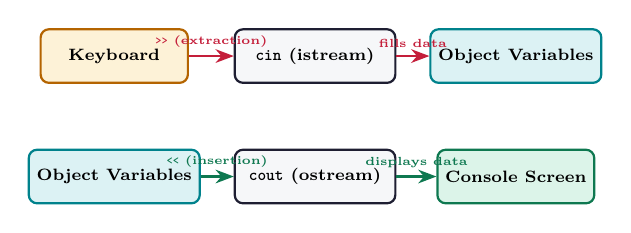
\begin{tikzpicture}[node distance=1.5cm, thick, scale=0.85, every node/.style={scale=0.85}]
  % Input Stream Flow
  \node[rectangle, draw=myamber, fill=hdramber, rounded corners=3pt, minimum width=2.2cm, minimum height=0.8cm, font=\scriptsize\bfseries] (keyboard) at (-3.5, 0.8) {Keyboard};
  \node[rectangle, draw=mydark, fill=mygray, rounded corners=3pt, minimum width=2.4cm, minimum height=0.8cm, font=\scriptsize\bfseries] (istream) at (-0.5, 0.8) {\texttt{cin} (istream)};
  \node[rectangle, draw=myteal, fill=hdrteal, rounded corners=3pt, minimum width=2.2cm, minimum height=0.8cm, font=\scriptsize\bfseries] (objIn) at (2.5, 0.8) {Object Variables};

  \draw[arrow, color=myred] (keyboard) -- (istream) node[midway, above, font=\tiny\bfseries] {\texttt{>>} (extraction)};
  \draw[arrow, color=myred] (istream) -- (objIn) node[midway, above, font=\tiny\bfseries] {fills data};

  % Output Stream Flow
  \node[rectangle, draw=myteal, fill=hdrteal, rounded corners=3pt, minimum width=2.2cm, minimum height=0.8cm, font=\scriptsize\bfseries] (objOut) at (-3.5, -1.0) {Object Variables};
  \node[rectangle, draw=mydark, fill=mygray, rounded corners=3pt, minimum width=2.4cm, minimum height=0.8cm, font=\scriptsize\bfseries] (ostream) at (-0.5, -1.0) {\texttt{cout} (ostream)};
  \node[rectangle, draw=mygreen, fill=hdrgreen, rounded corners=3pt, minimum width=2.2cm, minimum height=0.8cm, font=\scriptsize\bfseries] (console) at (2.5, -1.0) {Console Screen};

  \draw[arrow, color=mygreen] (objOut) -- (ostream) node[midway, above, font=\tiny\bfseries] {\texttt{<<} (insertion)};
  \draw[arrow, color=mygreen] (ostream) -- (console) node[midway, above, font=\tiny\bfseries] {displays data};
\end{tikzpicture}
\tcbset{colbacktitle=mgframe, coltitle=mydark}
\end{tcolorbox}

% ===============================================================================
\section{Type Conversions}
% ===============================================================================

C++ allows custom type conversions between primitive types and class objects.

\subsection{Basic Type to Class Type}
Handled automatically using a \textbf{parameterized constructor} inside the target class that accepts the basic type as an argument.
\begin{equation}
  \texttt{Time t1 = 95; // Invokes constructor Time(int) to convert minutes}
\end{equation}

\subsection{Class Type to Basic Type}
Accomplished by defining a \textbf{casting operator function} (conversion function) inside the class.
\textbf{Rules for Conversion Functions:}
\begin{itemize}[leftmargin=*, itemsep=2pt]
  \item It must be a class member function.
  \item It must not specify any return type (the return type is implicit from the operator's name).
  \item It must not accept any arguments.
\end{itemize}
\begin{equation}
  \text{Syntax: } \quad \texttt{operator}\;\text{Basic\_Type}\;() \quad \{ \quad \text{return}\;\text{value}; \quad \}
\end{equation}

\begin{tcolorbox}[examplebox, title={Code Example: Basic-to-Class and Class-to-Basic conversions}]
\begin{spacing}{1.0}
\begin{verbatim}
#include <iostream>
class Time {
private:
    int hours, minutes;
public:
    Time() : hours(0), minutes(0) {}
    
    // Basic to Class Conversion (Constructor)
    Time(int mins) {
        hours = mins / 60;
        minutes = mins % 60;
    }
    
    // Class to Basic Conversion (Casting Operator)
    operator int() {
        return (hours * 60) + minutes;
    }
    
    void display() {
        std::cout << hours << "h " << minutes << "m" << std::endl;
    }
};

int main() {
    // Basic -> Class
    Time t1 = 85; // Converts 85 (int) to 1h 25m (Time)
    t1.display(); // Prints: 1h 25m

    // Class -> Basic
    int totalMins = t1; // Converts Time to int using operator int()
    std::cout << "Total minutes = " << totalMins << std::endl; // 85
    return 0;
}
\end{verbatim}
\end{spacing}
\tcbset{colbacktitle=myamber, coltitle=white}
\end{tcolorbox}

% ===============================================================================
% MANDATORY QUICK REVISION PAGE
% ===============================================================================
\newpage
\begin{center}
  {\large\bfseries\color{myred} Quick Revision --- Module V}\\[3pt]
  {\small\color{mydark} Operator Overloading $|$ OE-EC604C}
\end{center}
\noindent{\color{myred}\rule{\linewidth}{1.2pt}}
\vspace{4pt}

\begin{tcolorbox}[formulabox, title={\textbf{Key Overloading Signatures}}]
\renewcommand{\arraystretch}{1.3}
\begin{tabularx}{\linewidth}{B{3.8cm} X}
Unary (Member)           & \texttt{Counter operator++() \{ /* prefix */ \}} \\[4pt]
Unary Postfix (Member)   & \texttt{Counter operator++(int) \{ /* dummy int parameter */ \}} \\[4pt]
Binary (Member)          & \texttt{Complex operator+(const Complex \&c) \{ /* 1 arg */ \}} \\[4pt]
Binary (Friend)          & \texttt{friend Complex operator+(Complex \&c1, Complex \&c2); // 2 args} \\[4pt]
Stream Insertion         & \texttt{friend ostream\& operator<<(ostream\& out, const MyClass \&obj);} \\[4pt]
Casting Function         & \texttt{operator float() \{ return data; \} // No return type specified}
\end{tabularx}
\end{tcolorbox}

\begin{tcolorbox}[defbox, title={\textbf{One-Line Definitions}}]
\begin{itemize}[leftmargin=*, itemsep=2.5pt, topsep=0pt]
  \item \textbf{Operator Overloading:} Assigning new functionalities to C++ operators when applied to class instances.
  \item \textbf{Stream Extraction (>>):} An overloaded operator used to extract formatted values from an input stream.
  \item \textbf{Stream Insertion (<<):} An overloaded operator used to insert formatted values into an output stream.
  \item \textbf{Conversion Operator:} A special class member function used to convert an object into another data type.
  \item \textbf{Prefix Operator:} An increment or decrement operator executed before evaluation of the expression.
  \item \textbf{Postfix Operator:} An increment or decrement operator executed after evaluation of the expression.
  \item \textbf{Basic to Class Conversion:} Converting standard types to user classes via parameterized constructors.
  \item \textbf{Class to Basic Conversion:} Converting classes to standard types via overloaded casting operators.
  \item \textbf{This Pointer:} An implicit pointer inside member functions that points to the calling object instance.
\end{itemize}
\end{tcolorbox}

\begin{tcolorbox}[exambox, title={\textbf{Frequently Asked / Viva Questions}}]
\begin{enumerate}[topsep=0pt, label=\textbf{Q\arabic*.}, itemsep=5pt]
  \item \Q{Which operators cannot be overloaded in C++? Why?}
    Operators like `.`, `.*`, `::`, `?:`, and `sizeof` cannot be overloaded to protect C++ syntax structures and core language bindings from corruption.
  \item \Q{Why does a postfix overloaded operator require a dummy `int` parameter?}
    The compiler uses the `int` parameter strictly as a signature flag to distinguish postfix calls (`obj++`) from prefix calls (`++obj`).
  \item \Q{Why must stream insertion (\texttt{<<}) and extraction (\texttt{>>}) operators be overloaded as friend functions?}
    The left-hand operand is `ostream` or `istream`, not our class object. Member functions require the left operand to be the class itself, so a friend function is mandatory.
  \item \Q{What is the difference in arguments between member and friend function operator overloading?}
    For binary operators: member functions take 1 argument (left operand is implicit); friend functions take 2 arguments explicitly. For unary operators: member functions take 0 arguments; friend functions take 1.
  \item \Q{Can we change the basic behaviors of operators (like changing $+$ to subtract)?}
    Yes, syntactically possible, but highly discouraged as it violates design clarity and makes code unreadable.
  \item \Q{What are the restrictions on type conversion functions?}
    They must be non-static class member functions, cannot have arguments, and must not specify a return type.
  \item \Q{Explain conversion from one class type to another class type.}
    This can be done using: (1) A constructor in the destination class that accepts the source class, or (2) A casting operator inside the source class that returns the destination class.
  \item \Q{Can we overload the assignment operator (\texttt{=}) as a friend function?}
    No. C++ rules mandate that \texttt{=}, \texttt{()}, \texttt{[]}, and \texttt{->} must be overloaded \textit{only} as member functions to prevent compiler syntax conflicts.
  \item \Q{What is the return type of stream insertion (\texttt{<<}) and extraction (\texttt{>>}) operators?}
    They return a reference to the stream object (`ostream\&` or `istream\&`). This allows chaining (e.g., `cout << a << b;`).
  \item \Q{Does operator overloading change the execution speed of a program?}
    No. Operator overloading is resolved at compile time (static binding), so it has zero runtime overhead compared to equivalent function calls.
  \item \Q{Is it possible to overload operators for standard types (like overloading $+$ for two integers)?}
    No. At least one operand must be a user-defined class or structure to prevent overriding standard arithmetic logic.
  \item \Q{Can we use default arguments in overloaded operators?}
    No, default arguments are not permitted in overloaded operators because they could conflict with the operator's expected arity.
\end{enumerate}
\tcbset{colbacktitle=mypurple, coltitle=white}
\end{tcolorbox}

\begin{tcolorbox}[tikzbox, title={Comparison: Member Functions vs. Friend Functions for Overloading}]
\renewcommand{\arraystretch}{1.45}
\par\noindent
\begin{tabularx}{\linewidth}{|B{3.2cm}|Y|Y|}
\hline
\textbf{Feature} & \textbf{\color{myteal}Member Function Overloading} & \textbf{\color{myamber}Friend Function Overloading} \\
\hline
\textbf{Implicit Operand} & Passes the left-hand operand implicitly via the \texttt{this} pointer. & No implicit operand. All operands must be explicitly declared in arguments. \\
\hline
\textbf{Left Operand Rule} & Left operand must strictly be an object of the defining class. & Left operand can be of any type (e.g., stream, primitive, other class). \\
\hline
\textbf{Number of Arguments} & Binary: 1 argument; Unary: 0 arguments. & Binary: 2 arguments; Unary: 1 argument. \\
\hline
\textbf{Class Encapsulation} & Maintains strict encapsulation boundaries. & Grants external function access (minor encapsulation bypass). \\
\hline
\textbf{Special Operators} & Mandatory for operators: \texttt{=}, \texttt{[]}, \texttt{()}, \texttt{->}. & Not allowed for: \texttt{=}, \texttt{[]}, \texttt{()}, \texttt{->}. \\
\hline
\end{tabularx}
\end{tcolorbox}


% -- Module 6 -----------------------------------------------------------------
\modulestart{6}{Fundamentals of Inheritance \& Derivation Levels}

\section{Fundamentals of Inheritance \& Derivation Levels}
% ===============================================================================

Inheritance is the mechanism by which a new class (derived class) is built from an existing class (base class), inheriting its properties and behaviors. This promotes code reusability.

\subsection{Base and Derived Classes}
A derived class inherits members of a base class. The visibility of inherited members depends on the \textbf{inheritance access level} declared:
\begin{enumerate}[label=\textbf{\arabic*.}, leftmargin=*, itemsep=2.5pt]
  \item \textbf{Public Derivation (\texttt{class Derived : public Base}):} 
    \begin{itemize}[leftmargin=1.5em, itemsep=1pt, topsep=1pt]
      \item Public base members become \textbf{public} in the derived class.
      \item Protected base members become \textbf{protected} in the derived class.
      \item Private base members are \textbf{never accessible} directly (can only be accessed via public/protected base functions).
    \end{itemize}
  \item \textbf{Protected Derivation (\texttt{class Derived : protected Base}):} 
    \begin{itemize}[leftmargin=1.5em, itemsep=1pt, topsep=1pt]
      \item Public and protected base members become \textbf{protected} in the derived class.
    \end{itemize}
  \item \textbf{Private Derivation (\texttt{class Derived : private Base}):} 
    \begin{itemize}[leftmargin=1.5em, itemsep=1pt, topsep=1pt]
      \item Public and protected base members become \textbf{private} in the derived class.
    \end{itemize}
\end{enumerate}

\subsection{Types of Inheritance}
C++ supports five distinct inheritance topologies:
\begin{itemize}[leftmargin=*, itemsep=3pt]
  \item \textbf{Single Inheritance:} One base class, one derived class.
  \item \textbf{Multilevel Inheritance:} A class is derived from another derived class (e.g., \texttt{A -> B -> C}).
  \item \textbf{Multiple Inheritance:} A derived class has more than one base class (e.g., \texttt{A} and \texttt{B} inherited by \texttt{C}).
  \item \textbf{Hierarchical Inheritance:} Multiple derived classes inherit from a single base class.
  \item \textbf{Hybrid Inheritance:} A combination of two or more inheritance types (e.g., multiple + hierarchical).
\end{itemize}

% ===============================================================================
\section{Constructor \& Destructor Execution Sequence}
% ===============================================================================

When a derived class object is instantiated, constructors are executed along the inheritance chain to ensure that the entire object is initialized.

\subsection{Invocation Sequence Rules}
\begin{itemize}[leftmargin=*, itemsep=3pt]
  \item \textbf{Constructors:} Executed from \textbf{top to bottom} along the class hierarchy. The base class constructor is executed first, followed by the derived class constructor.
  \item \textbf{Destructors:} Executed in the \textbf{exact reverse order} (bottom to top).
  \item \textbf{Initializer Lists:} Parameterized base constructors must be explicitly called using the derived class constructor's member initialization list.
\end{itemize}

\begin{tcolorbox}[examplebox, title={Code Example: Invocation of parameterized base constructors}]
\begin{spacing}{1.0}
\begin{verbatim}
#include <iostream>
class Base {
protected:
    int baseVal;
public:
    Base(int val) : baseVal(val) {
        std::cout << "Base Constructor: " << baseVal << std::endl;
    }
    ~Base() {
        std::cout << "Base Destructor" << std::endl;
    }
};

class Derived : public Base {
private:
    int derivedVal;
public:
    // Call base constructor explicitly in initialization list
    Derived(int bVal, int dVal) : Base(bVal), derivedVal(dVal) {
        std::cout << "Derived Constructor: " << derivedVal << std::endl;
    }
    ~Derived() {
        std::cout << "Derived Destructor" << std::endl;
    }
};
\end{verbatim}
\end{spacing}
\tcbset{colbacktitle=myamber, coltitle=white}
\end{tcolorbox}

% ===============================================================================
\section{The Diamond Inheritance Ambiguity}
% ===============================================================================

Multipath inheritance can result in a duplicate copy conflict known as the \textbf{Diamond Problem}.

\subsection{The Diamond Problem and Virtual Base Classes}
Consider class \texttt{D} inheriting from classes \texttt{B} and \texttt{C}, which both inherit from class \texttt{A}.
If \texttt{A} contains a member \texttt{x}, \texttt{D} receives two separate copies of \texttt{x} (one via \texttt{B} and one via \texttt{C}). Any reference to \texttt{x} inside \texttt{D} is flagged as \textbf{ambiguous} by the compiler.
\begin{tcolorbox}[defbox]
\textbf{Virtual Base Class:} By declaring the base class \texttt{A} as \texttt{virtual} during derivation in \texttt{B} and \texttt{C}, the compiler ensures that only one shared instance of class \texttt{A} is created in memory, resolving all inheritance path ambiguities.
\end{tcolorbox}

\begin{tcolorbox}[tikzbox, title={Diamond Inheritance Path Topologies}]
\centering
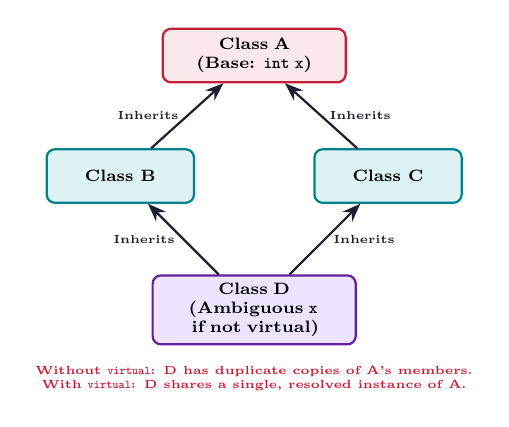
\begin{tikzpicture}[node distance=1.5cm, thick, scale=0.85, every node/.style={scale=0.85}]
  % Top Node
  \node[rectangle, draw=myred, fill=hdrred, rounded corners=3pt, align=center, text width=2.5cm, minimum height=0.8cm, font=\scriptsize\bfseries] (baseA) at (0, 1.8) {Class A \\ (Base: \texttt{int x})};

  % Middle Nodes
  \node[rectangle, draw=myteal, fill=hdrteal, rounded corners=3pt, minimum width=2.2cm, minimum height=0.8cm, font=\scriptsize\bfseries] (derB) at (-2.0, 0) {Class B};
  \node[rectangle, draw=myteal, fill=hdrteal, rounded corners=3pt, minimum width=2.2cm, minimum height=0.8cm, font=\scriptsize\bfseries] (derC) at (2.0, 0) {Class C};

  % Bottom Node
  \node[rectangle, draw=mypurple, fill=hdrpurple, rounded corners=3pt, align=center, text width=2.8cm, minimum height=1.0cm, font=\scriptsize\bfseries] (derD) at (0, -2.0) {Class D \\ (Ambiguous \texttt{x} if not virtual)};

  % Paths
  \draw[arrow] (derB) -- (baseA) node[midway, left, font=\tiny\bfseries] {Inherits};
  \draw[arrow] (derC) -- (baseA) node[midway, right, font=\tiny\bfseries] {Inherits};
  \draw[arrow] (derD) -- (derB) node[midway, left, font=\tiny\bfseries] {Inherits};
  \draw[arrow] (derD) -- (derC) node[midway, right, font=\tiny\bfseries] {Inherits};

  % Text indicators
  \node[below=0.15cm of derD, font=\tiny\bfseries\color{myred}, align=center] {Without \texttt{virtual}: D has duplicate copies of A's members.\\With \texttt{virtual}: D shares a single, resolved instance of A.};
\end{tikzpicture}
\tcbset{colbacktitle=mgframe, coltitle=mydark}
\end{tcolorbox}

\begin{tcolorbox}[examplebox, title={Code Example: Resolving Diamond Problem using Virtual Base Class}]
\begin{spacing}{1.0}
\begin{verbatim}
#include <iostream>
class A {
public:
    int x;
};

// Declare B and C with virtual public inheritance
class B : virtual public A {
public:
    int y;
};

class C : virtual public A {
public:
    int z;
};

class D : public B, public C {
public:
    int sum;
    void show() {
        x = 10; // Ambiguous without virtual keyword! Now resolved.
        y = 20;
        z = 30;
        sum = x + y + z;
        std::cout << "Sum = " << sum << std::endl;
    }
};
\end{verbatim}
\end{spacing}
\tcbset{colbacktitle=myamber, coltitle=white}
\end{tcolorbox}

% ===============================================================================
\section{Containership vs. Inheritance}
% ===============================================================================

To design clean systems, software developers must choose the correct structural relationship between classes:
\begin{itemize}[leftmargin=*, itemsep=3pt]
  \item \textbf{Inheritance (\texttt{is-a} relationship):} A derived class inherits properties of the base class. E.g., a \texttt{Car} \textbf{is a} \texttt{Vehicle}.
  \item \textbf{Containership (\texttt{has-a} relationship):} An object of one class is embedded as a data member inside another class. E.g., a \texttt{Car} \textbf{has an} \texttt{Engine}.
\end{itemize}

% ===============================================================================
% MANDATORY QUICK REVISION PAGE
% ===============================================================================
\newpage
\begin{center}
  {\large\bfseries\color{myred} Quick Revision --- Module VI}\\[3pt]
  {\small\color{mydark} Inheritance $|$ OE-EC604C}
\end{center}
\noindent{\color{myred}\rule{\linewidth}{1.2pt}}
\vspace{4pt}

\begin{tcolorbox}[formulabox, title={\textbf{Access Control Table under Derivation}}]
\renewcommand{\arraystretch}{1.3}
\par\noindent
\begin{tabularx}{\linewidth}{|B{2.8cm}|Y|Y|Y|}
\hline
\textbf{Base Member} & \textbf{Public Derivation} & \textbf{Protected Derivation} & \textbf{Private Derivation} \\
\hline
\textbf{Private}     & Not Accessible & Not Accessible & Not Accessible \\
\hline
\textbf{Protected}   & Protected in Derived & Protected in Derived & Private in Derived \\
\hline
\textbf{Public}      & Public in Derived & Protected in Derived & Private in Derived \\
\hline
\end{tabularx}
\end{tcolorbox}

\begin{tcolorbox}[defbox, title={\textbf{One-Line Definitions}}]
\begin{itemize}[leftmargin=*, itemsep=2.5pt, topsep=0pt]
  \item \textbf{Inheritance:} The mechanism of deriving a new class from an existing base class to reuse code.
  \item \textbf{Base Class:} The existing class from which features are inherited.
  \item \textbf{Derived Class:} The new class that inherits features from one or more base classes.
  \item \textbf{Diamond Problem:} An ambiguity issue where a derived class inherits duplicate members of a grandparent class through two distinct paths.
  \item \textbf{Virtual Base Class:} A base class declared virtual to ensure only one instance is shared in multipath inheritance.
  \item \textbf{Containership:} Embedding an object of one class as a member variable inside another class (Composition).
  \item \textbf{Initialization List (Base):} The derived constructor syntax used to pass arguments to base class constructors.
  \item \textbf{Is-A Relationship:} Logical relationship modeled by class inheritance (e.g., Dog is-a Mammal).
  \item \textbf{Has-A Relationship:} Logical relationship modeled by class containership (e.g., Dog has-a Tail).
\end{itemize}
\end{tcolorbox}

\begin{tcolorbox}[exambox, title={\textbf{Frequently Asked / Viva Questions}}]
\begin{enumerate}[topsep=0pt, label=\textbf{Q\arabic*.}, itemsep=5pt]
  \item \Q{Why are private base class members not accessible in derived classes?}
    This maintains the privacy boundaries of class design. If derived classes could access private members directly, encapsulation could be easily broken.
  \item \Q{Explain why virtual inheritance is necessary to solve the Diamond Problem.}
    Virtual inheritance directs the compiler to build only one shared instance of the grandparent class, resolving lookup ambiguity for its members.
  \item \Q{What is the execution order of constructors in multiple inheritance?}
    Base constructors are executed in the order they are listed in the inheritance declaration, NOT the order they appear in the initializer list. E.g., `class D : public B, public C` calls B's constructor first, then C's.
  \item \Q{Which class constructor is executed first in multilevel inheritance?}
    The absolute root base class constructor is executed first, followed by intermediate bases, ending at the leaf derived class.
  \item \Q{Does a derived class inherit the constructor of the base class?}
    No. Constructors are class-specific and are not inherited. A derived class must define its own constructors or use the default constructor.
  \item \Q{Can we declare a destructor virtual? Why?}
    Yes, virtual destructors are mandatory when deleting derived objects via base pointers to ensure derived resource cleanup.
  \item \Q{What is the difference between multiple inheritance and hybrid inheritance?}
    Multiple inheritance involves deriving from 2+ distinct base classes. Hybrid inheritance combines multiple topologic models (like multiple and multilevel).
  \item \Q{How does containership differ from private inheritance?}
    Containership embeds objects as members, restricting them to public APIs. Private inheritance makes base members private, permitting code access but hiding public APIs from external callers.
  \item \Q{What happens if base and derived classes declare members with the same name?}
    The derived member hides the base member. The base member can still be accessed using the scope resolution operator: `BaseClass::memberName`.
  \item \Q{Can a class inherit from itself in C++?}
    No, circular or self-inheritance (e.g., `class A : public A`) is syntactically invalid and causes compile errors.
  \item \Q{Why does virtual inheritance require base class constructors to be called by the most derived class?}
    Since the base class instance is shared, intermediate derived classes cannot initialize it independently. The most derived class constructor executes its initialization.
  \item \Q{How does the visibility level of inheritance affect derived class inheritance hierarchies?}
    Private inheritance prevents downstream subclasses from accessing grandparent class members, whereas public/protected inheritances allow subclass access.
\end{enumerate}
\tcbset{colbacktitle=mypurple, coltitle=white}
\end{tcolorbox}

\begin{tcolorbox}[tikzbox, title={Comparison: Multiple Inheritance vs. Hybrid Inheritance}]
\renewcommand{\arraystretch}{1.45}
\par\noindent
\begin{tabularx}{\linewidth}{|B{3.2cm}|Y|Y|}
\hline
\textbf{Feature} & \textbf{\color{myteal}Multiple Inheritance} & \textbf{\color{myamber}Hybrid Inheritance} \\
\hline
\textbf{Structure} & A single subclass derives directly from two or more parent classes. & Combines two or more basic inheritance shapes (e.g., hierarchic, multilevel, multiple). \\
\hline
\textbf{Diamond Risk} & None, unless parent classes share a common grandparent class. & High. Multipath inheritance frequently creates diamond path ambiguities. \\
\hline
\textbf{Complexity} & Moderate. Simple to resolve using qualifiers. & High. Requires virtual inheritance declaration to resolve duplicate members. \\
\hline
\textbf{Design Goal} & Merging features from multiple independent source interfaces. & Modeling complex real-world classification hierarchies. \\
\hline
\end{tabularx}
\tcbset{colbacktitle=mgframe, coltitle=mydark}
\end{tcolorbox}


% -- Module 7 -----------------------------------------------------------------
\modulestart{7}{Fundamentals of Polymorphism}

\section{Fundamentals of Polymorphism}
% ===============================================================================

Polymorphism ("many forms") allows a single interface to represent different underlying forms (behaviors). In C++, it is broadly classified into compile-time and run-time polymorphism.

\subsection{Pointers to Objects and Polymorphic Assignments}
Pointers can store the addresses of objects. In inheritance hierarchies, C++ supports upcasting:
\begin{tcolorbox}[defbox]
\textbf{Upcasting Rule:} A base class pointer can point to a derived class object without explicit typecasting. However, using this pointer, we can only access base class members, unless the functions are virtual.
\end{tcolorbox}
\begin{equation}
  \texttt{Base* ptr = new Derived(); // Polymorphic Assignment}
\end{equation}

\subsection{The \texorpdfstring{\texttt{this}}{this} Pointer}
The \texttt{this} pointer is an implicit parameter passed to all non-static member functions.
\textbf{Characteristics:}
\begin{itemize}[leftmargin=*, itemsep=2pt]
  \item It stores the address of the calling object.
  \item Used to resolve naming conflicts between member variables and parameters: \texttt{this->data = data;}.
  \item Used to return the calling object itself to enable \textbf{method chaining}: \texttt{return *this;}.
\end{itemize}

% ===============================================================================
\section{Compile-Time vs. Run-Time Polymorphism}
% ===============================================================================

The primary distinction lies in when the compiler resolves function invocations.

\subsection{Virtual Functions and Late Binding}
By prefixing a base class function declaration with the \texttt{virtual} keyword, we tell the compiler to resolve function calls at \textbf{run time} (late binding) based on the type of the object pointed to, rather than the type of the pointer.

\textbf{Mechanism of Late Binding (V-Table and V-Ptr):}
\begin{enumerate}[label=\textbf{\arabic*.}, leftmargin=*, itemsep=2.5pt]
  \item \textbf{V-Ptr (Virtual Pointer):} Every object of a class containing virtual functions is automatically allocated a hidden pointer field (\texttt{vptr}) pointing to its class's V-Table.
  \item \textbf{V-Table (Virtual Method Table):} A static table compiled for each class containing function addresses for all its virtual functions.
\end{enumerate}

\begin{tcolorbox}[tikzbox, title={Virtual Method Table (V-Table) Mapping Layout}]
\centering
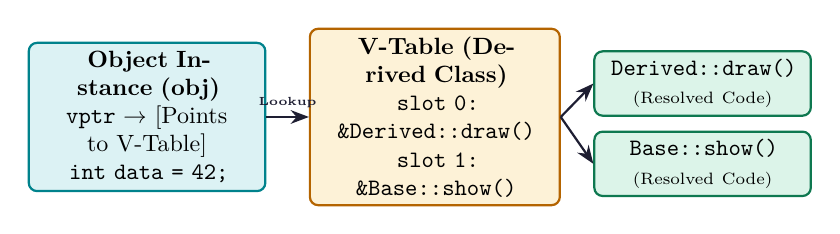
\begin{tikzpicture}[node distance=1.5cm, thick, scale=0.85, every node/.style={scale=0.85}]
  % Object Instance
  \node[rectangle, draw=myteal, fill=hdrteal, rounded corners=3pt, text width=3.3cm, align=center, minimum height=1.4cm] (obj) at (-3.5, 0) {
    \textbf{Object Instance (obj)}\\
    \texttt{vptr} $\rightarrow$ [Points to V-Table]\\
    \texttt{int data = 42;}
  };

  % V-Table
  \node[rectangle, draw=myamber, fill=hdramber, rounded corners=3pt, text width=3.5cm, align=center, minimum height=1.4cm] (vtable) at (0.8, 0) {
    \textbf{V-Table (Derived Class)}\\
    \texttt{slot 0:} \texttt{\&Derived::draw()}\\
    \texttt{slot 1:} \texttt{\&Base::show()}
  };

  % Code Segment
  \node[rectangle, draw=mygreen, fill=hdrgreen, rounded corners=3pt, text width=3.0cm, align=center, minimum height=0.7cm] (func0) at (4.8, 0.5) {
    \texttt{Derived::draw()}\\
    \scriptsize{(Resolved Code)}
  };
  \node[rectangle, draw=mygreen, fill=hdrgreen, rounded corners=3pt, text width=3.0cm, align=center, minimum height=0.7cm] (func1) at (4.8, -0.7) {
    \texttt{Base::show()}\\
    \scriptsize{(Resolved Code)}
  };

  % Arrows
  \draw[arrow] (obj.east) -- (vtable.west) node[midway, above, font=\tiny\bfseries] {Lookup};
  \draw[arrow] (vtable.east) -- (func0.west);
  \draw[arrow] (vtable.east) -- (func1.west);
\end{tikzpicture}
\tcbset{colbacktitle=mgframe, coltitle=mydark}
\end{tcolorbox}

\begin{tcolorbox}[examplebox, title={Code Example: Runtime polymorphism using base pointer arrays}]
\begin{spacing}{1.0}
\begin{verbatim}
#include <iostream>
class Shape {
public:
    virtual void draw() { // Virtual function
        std::cout << "Drawing generic shape" << std::endl;
    }
    virtual ~Shape() {} // Virtual destructor
};

class Circle : public Shape {
public:
    void draw() override { // Overridden function
        std::cout << "Drawing Circle" << std::endl;
    }
};

class Box : public Shape {
public:
    void draw() override {
        std::cout << "Drawing Box" << std::endl;
    }
};

int main() {
    Shape* shapes[2];
    shapes[0] = new Circle();
    shapes[1] = new Box();
    
    for(int i = 0; i < 2; i++) {
        shapes[i]->draw(); // Late binding: calls appropriate draw()
        delete shapes[i];
    }
    return 0;
}
\end{verbatim}
\end{spacing}
\tcbset{colbacktitle=myamber, coltitle=white}
\end{tcolorbox}

% ===============================================================================
\section{Pure Virtual Functions and Abstract Classes}
% ===============================================================================

Sometimes, a base class is so generic that it cannot provide any logical default implementation for its virtual functions.

\subsection{Pure Virtual Functions}
\begin{tcolorbox}[defbox]
\textbf{Pure Virtual Function:} A virtual function declared in a base class with no implementation, represented by assigning \texttt{= 0} at its declaration.
\end{tcolorbox}
\begin{equation}
  \text{Declaration: } \quad \texttt{virtual}\;\text{Return\_Type}\;\text{FuncName}(\text{Args}) = 0;
\end{equation}

\subsection{Abstract Classes}
A class containing at least one pure virtual function is an \textbf{Abstract Class}.
\textbf{Key Characteristics:}
\begin{itemize}[leftmargin=*, itemsep=2.5pt]
  \item Instantiation: Abstract classes cannot be used to instantiate objects. E.g., \texttt{Employee emp;} is a compile error.
  \item Subclassing: Derived classes must override \textbf{all} inherited pure virtual functions to become concrete classes. Failure to do so makes the derived class abstract as well.
\end{itemize}

\begin{tcolorbox}[examplebox, title={Code Example: Abstract Employee base class}]
\begin{spacing}{1.0}
\begin{verbatim}
#include <iostream>
#include <string>
class Employee {
protected:
    std::string name;
public:
    Employee(std::string n) : name(n) {}
    virtual double calculateSalary() = 0; // Pure virtual function
    virtual void display() {
        std::cout << "Employee: " << name << std::endl;
    }
    virtual ~Employee() {}
};

class FullTimeEmployee : public Employee {
private:
    double monthlySalary;
public:
    FullTimeEmployee(std::string n, double s) : Employee(n), monthlySalary(s) {}
    double calculateSalary() override { return monthlySalary; }
};
\end{verbatim}
\end{spacing}
\tcbset{colbacktitle=myamber, coltitle=white}
\end{tcolorbox}

% ===============================================================================
\section{Virtual Destructors \& Memory Leaks}
% ===============================================================================

When destroying dynamically allocated derived class objects through base class pointers, memory leaks will occur unless the base class destructor is virtual.

\subsection{Destructor Call Failures}
If the base class destructor is \textbf{non-virtual}, the compiler binds the destructor call to the base pointer type at compile time.
As a result, only the base class destructor executes. The derived class destructor never runs, leaving any heap allocations or handles inside the derived class unreleased.

\begin{tcolorbox}[examplebox, title={Code Example: Memory leak prevention via Virtual Destructors}]
\begin{spacing}{1.0}
\begin{verbatim}
#include <iostream>
class Base {
public:
    Base() { std::cout << "Base Constructor" << std::endl; }
    // Declaring destructor virtual guarantees derived deallocation
    virtual ~Base() { std::cout << "Base Destructor" << std::endl; }
};

class Derived : public Base {
private:
    int* data;
public:
    Derived() {
        std::cout << "Derived Constructor" << std::endl;
        data = new int[100]; // Heap allocation
    }
    ~Derived() {
        std::cout << "Derived Destructor (Releasing Heap)" << std::endl;
        delete[] data; // Releases resource safely
    }
};

int main() {
    Base* ptr = new Derived();
    delete ptr; // Triggers Derived destructor then Base destructor
    return 0;
}
\end{verbatim}
\end{spacing}
\tcbset{colbacktitle=myamber, coltitle=white}
\end{tcolorbox}

% ===============================================================================
% MANDATORY QUICK REVISION PAGE
% ===============================================================================
\newpage
\begin{center}
  {\large\bfseries\color{myred} Quick Revision --- Module VII}\\[3pt]
  {\small\color{mydark} Polymorphism $|$ OE-EC604C}
\end{center}
\noindent{\color{myred}\rule{\linewidth}{1.2pt}}
\vspace{4pt}

\begin{tcolorbox}[formulabox, title={\textbf{Key Polymorphic Syntax}}]
\renewcommand{\arraystretch}{1.3}
\begin{tabularx}{\linewidth}{B{3.8cm} X}
Virtual Declaration      & \texttt{virtual void print(); // Inside base class declaration} \\[4pt]
Override Qualifier       & \texttt{void print() override; // Inside derived class (C++11)} \\[4pt]
Pure Virtual Function    & \texttt{virtual void process() = 0; // Defines abstract interface} \\[4pt]
Virtual Destructor       & \texttt{virtual \textasciitilde Base() \{ /* virtual base destructor */ \}}
\end{tabularx}
\end{tcolorbox}

\begin{tcolorbox}[defbox, title={\textbf{One-Line Definitions}}]
\begin{itemize}[leftmargin=*, itemsep=2.5pt, topsep=0pt]
  \item \textbf{Polymorphism:} The ability of different classes to respond uniquely to identical message calls.
  \item \textbf{Virtual Function:} A class member function overridden in derived classes to ensure late binding execution.
  \item \textbf{Late Binding:} Resolving function calls at run time based on the active object's type.
  \item \textbf{V-Table:} A compiler-generated static lookup table storing virtual function addresses for a class.
  \item \textbf{V-Ptr:} An object instance pointer referencing the V-Table allocated during object instantiation.
  \item \textbf{Pure Virtual Function:} An abstract base method initialized to \texttt{= 0} that derived classes must override.
  \item \textbf{Abstract Class:} A class containing pure virtual methods that cannot be instantiated.
  \item \textbf{Virtual Destructor:} A base class destructor configured to trigger proper intermediate subclass destructor sequences.
  \item \textbf{This Pointer:} An implicit member pointer storing the memory address of the calling object.
\end{itemize}
\end{tcolorbox}

\begin{tcolorbox}[exambox, title={\textbf{Frequently Asked / Viva Questions}}]
\begin{enumerate}[topsep=0pt, label=\textbf{Q\arabic*.}, itemsep=5pt]
  \item \Q{What is the difference between early binding and late binding?}
    Early binding (compile time) resolves function addresses using pointer types. Late binding (run time) resolves addresses using the pointed-to object type via the V-Table lookup.
  \item \Q{Can we declare a virtual function inside a structure (\texttt{struct})?}
    Yes. Structures in C++ are identical to classes but use public access by default. They support the `virtual` keyword and inheritance.
  \item \Q{What is the size impact of adding virtual functions to a class?}
    It adds the size of a single pointer (`vptr`) to every object instance (typically 4 bytes on 32-bit and 8 bytes on 64-bit systems), regardless of how many virtual functions are defined.
  \item \Q{Can a class have virtual static member functions?}
    No. Static member functions are class-wide and do not bind to object instances. Since they lack a `this` pointer and `vptr` links, they cannot be virtual.
  \item \Q{Can we override private virtual functions in C++?}
    Yes. The derived class can override private base virtual functions. Access levels only restrict calling permissions, not inheritance resolution.
  \item \Q{What is the difference between overloading and overriding?}
    Overloading occurs within the same class scope (same name, different arguments). Overriding occurs between base and derived classes (same name, identical arguments, uses `virtual`).
  \item \Q{Can an abstract class have constructors?}
    Yes. An abstract class cannot be instantiated directly, but its constructors run during derived class constructor sequences to initialize inherited data members.
  \item \Q{Why does a constructor declare base classes virtual during multiple derivations?}
    To bypass duplicate grandparent member allocations in hybrid structures (solving the Diamond Problem).
  \item \Q{What happens if we forget to declare base destructors virtual?}
    Deleting derived class instances through base class pointers only calls the base destructor, leaking derived heap resources.
  \item \Q{What is a pure abstract class or interface?}
    A class that contains \textit{only} pure virtual functions and no data members. It acts purely as a behavior contract.
  \item \Q{Can we call a virtual function from a constructor or destructor?}
    Yes, but early binding is used. It calls the local class's implementation, not the derived class's version, because the derived object is not yet fully constructed or is already destroyed.
  \item \Q{What is the purpose of the `override` keyword in C++11?}
    It instructs the compiler to verify that the function matches a virtual base class signature, preventing signature mismatch errors.
\end{enumerate}
\tcbset{colbacktitle=mypurple, coltitle=white}
\end{tcolorbox}

\begin{tcolorbox}[tikzbox, title={Comparison: Compile-Time vs. Run-Time Polymorphism}]
\renewcommand{\arraystretch}{1.45}
\par\noindent
\begin{tabularx}{\linewidth}{|B{3.2cm}|Y|Y|}
\hline
\textbf{Feature} & \textbf{\color{myteal}Compile-Time Polymorphism} & \textbf{\color{myamber}Run-Time Polymorphism} \\
\hline
\textbf{Binding Time} & resolved at compile time (Static Binding / Early Binding). & resolved at run time (Dynamic Binding / Late Binding). \\
\hline
\textbf{Mechanism} & Function Overloading and Operator Overloading. & Virtual Functions. \\
\hline
\textbf{Speed} & Fast execution (no run-time address lookup overhead). & Slightly slower (requires dereferencing the V-Ptr and V-Table lookup). \\
\hline
\textbf{Flexibility} & Fixed logic flow determined during compilation. & Highly flexible; handles new derived classes at runtime. \\
\hline
\textbf{Requirements} & Unique signatures (number/type of parameters). & Identical signatures; requires base pointer/reference interface. \\
\hline
\end{tabularx}
\tcbset{colbacktitle=mgframe, coltitle=mydark}
\end{tcolorbox}


% -- Module 8 -----------------------------------------------------------------
\modulestart{8}{C++ File Streams Hierarchy}

\section{C++ File Streams Hierarchy}
% ===============================================================================

C++ models file input and output operations using a system of classes inherited from basic stream classes.

\subsection{The Stream Class Hierarchy}
All stream classes are derived from a common virtual base class \texttt{ios}. The main classes used for file operations are:
\begin{itemize}[leftmargin=*, itemsep=3.5pt]
  \item \textbf{\texttt{ifstream}:} Input file stream. Derived from \texttt{istream}, used for reading files.
  \item \textbf{\texttt{ofstream}:} Output file stream. Derived from \texttt{ostream}, used for creating and writing files.
  \item \textbf{\texttt{fstream}:} Input/Output file stream. Derived from \texttt{iostream}, used for simultaneous reading and writing operations.
\end{itemize}

\begin{tcolorbox}[tikzbox, title={C++ Stream Class Hierarchy Topology}]
\centering
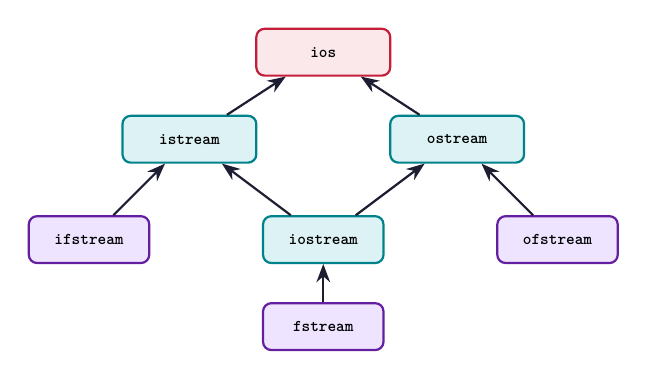
\begin{tikzpicture}[node distance=1.2cm, thick, scale=0.85, every node/.style={scale=0.85}]
  % Root node
  \node[rectangle, draw=myred, fill=hdrred, rounded corners=3pt, minimum width=2.0cm, minimum height=0.7cm, font=\scriptsize\bfseries] (ios) at (0, 2.0) {\texttt{ios}};

  % Intermediate nodes
  \node[rectangle, draw=myteal, fill=hdrteal, rounded corners=3pt, minimum width=2.0cm, minimum height=0.7cm, font=\scriptsize\bfseries] (istream) at (-2.0, 0.7) {\texttt{istream}};
  \node[rectangle, draw=myteal, fill=hdrteal, rounded corners=3pt, minimum width=2.0cm, minimum height=0.7cm, font=\scriptsize\bfseries] (ostream) at (2.0, 0.7) {\texttt{ostream}};

  % Derived stream classes
  \node[rectangle, draw=mypurple, fill=hdrpurple, rounded corners=3pt, minimum width=1.8cm, minimum height=0.7cm, font=\scriptsize\bfseries] (ifstream) at (-3.5, -0.8) {\texttt{ifstream}};
  \node[rectangle, draw=myteal, fill=hdrteal, rounded corners=3pt, minimum width=1.8cm, minimum height=0.7cm, font=\scriptsize\bfseries] (iostream) at (0, -0.8) {\texttt{iostream}};
  \node[rectangle, draw=mypurple, fill=hdrpurple, rounded corners=3pt, minimum width=1.8cm, minimum height=0.7cm, font=\scriptsize\bfseries] (ofstream) at (3.5, -0.8) {\texttt{ofstream}};

  % Bottom fstream node
  \node[rectangle, draw=mypurple, fill=hdrpurple, rounded corners=3pt, minimum width=1.8cm, minimum height=0.7cm, font=\scriptsize\bfseries] (fstream) at (0, -2.1) {\texttt{fstream}};

  % Inheritance arrows
  \draw[arrow] (istream) -- (ios);
  \draw[arrow] (ostream) -- (ios);
  \draw[arrow] (ifstream) -- (istream);
  \draw[arrow] (iostream) -- (istream);
  \draw[arrow] (iostream) -- (ostream);
  \draw[arrow] (ofstream) -- (ostream);
  \draw[arrow] (fstream) -- (iostream);
\end{tikzpicture}
\tcbset{colbacktitle=mgframe, coltitle=mydark}
\end{tcolorbox}

% ===============================================================================
\section{Opening \& Closing Files}
% ===============================================================================

Files can be opened in two ways: using the constructor or using the \texttt{open()} method.

\subsection{File Open Methods}
\begin{enumerate}[label=\textbf{\arabic*.}, leftmargin=*, itemsep=3pt]
  \item \textbf{Using Constructor:} Best when managing a single file throughout the stream's lifetime.
    \begin{equation}
      \texttt{ofstream outFile("data.txt"); // Opens file automatically}
    \end{equation}
  \item \textbf{Using \texttt{open()} method:} Best when reusing a single stream object to access multiple files sequentially.
    \begin{equation}
      \texttt{ifstream inFile; inFile.open("data.txt");}
    \end{equation}
\end{enumerate}

\subsection{File Modes}
File modes specify the access permissions and options for opening files.
\renewcommand{\arraystretch}{1.3}
\par\noindent
\begin{tabularx}{\linewidth}{|B{3.4cm}|Y|}
\hline
\textbf{File Mode Constant} & \textbf{Description} \\
\hline
\texttt{ios::in} & Opens the file for reading (default for \texttt{ifstream}). \\
\hline
\texttt{ios::out} & Opens the file for writing (default for \texttt{ofstream}). Erases existing content. \\
\hline
\texttt{ios::app} & Append mode. All write operations occur at the end of the file. \\
\hline
\texttt{ios::ate} & Opens the file and moves the pointer to the end of the file. \\
\hline
\texttt{ios::binary} & Opens the file in binary mode (instead of default text mode). \\
\hline
\end{tabularx}

% ===============================================================================
\section{File Pointers and Seek Operations}
% ===============================================================================

Each file stream object maintains file pointers that keep track of reading or writing locations.

\subsection{Seek and Tell Functions}
\begin{itemize}[leftmargin=*, itemsep=3.5pt]
  \item \textbf{\texttt{seekg()}:} Moves the \textbf{get} (read) pointer to a new position.
  \item \textbf{\texttt{seekp()}:} Moves the \textbf{put} (write) pointer to a new position.
  \item \textbf{\texttt{tellg()}:} Returns the current offset position of the get pointer.
  \item \textbf{\texttt{tellp()}:} Returns the current offset position of the put pointer.
\end{itemize}

\begin{tcolorbox}[defbox, title={\textbf{Seek Syntax Parameters}}]
\begin{align}
  &\texttt{stream.seekg(offset, direction);} \\
  &\text{Where direction can be: } \texttt{ios::beg} \quad \text{or} \quad \texttt{ios::cur} \quad \text{or} \quad \texttt{ios::end}
\end{align}
\end{tcolorbox}

\begin{tcolorbox}[tikzbox, title={File Pointer Position and Offset Directions}]
\centering
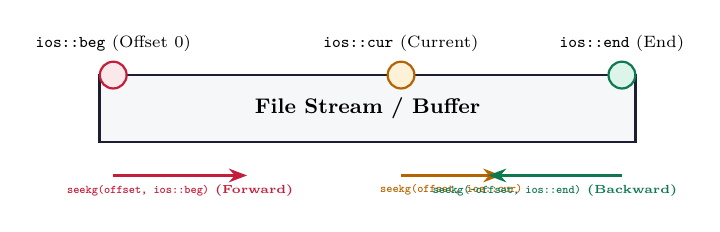
\begin{tikzpicture}[node distance=1.5cm, thick, scale=0.85, every node/.style={scale=0.85}]
  % File Buffer box
  \draw[draw=mydark, fill=mygray, line width=1.0pt] (-4.0, 0.5) rectangle (4.0, -0.5);
  \node[font=\small\bfseries] at (0, 0) {File Stream / Buffer};

  % Anchor Points
  \node[circle, draw=myred, fill=hdrred, minimum size=0.4cm, label=above:{\scriptsize\texttt{ios::beg} (Offset 0)}] (beg) at (-3.8, 0.5) {};
  \node[circle, draw=myamber, fill=hdramber, minimum size=0.4cm, label=above:{\scriptsize\texttt{ios::cur} (Current)}] (cur) at (0.5, 0.5) {};
  \node[circle, draw=mygreen, fill=hdrgreen, minimum size=0.4cm, label=above:{\scriptsize\texttt{ios::end} (End)}] (end) at (3.8, 0.5) {};

  % Seek Operations
  \draw[arrow, color=myred] (-3.8, -1.0) -- (-1.8, -1.0) node[midway, below, font=\tiny\bfseries] {\texttt{seekg(offset, ios::beg)} (Forward)};
  \draw[arrow, color=myamber] (0.5, -1.0) -- (2.0, -1.0) node[midway, below, font=\tiny\bfseries] {\texttt{seekg(offset, ios::cur)}};
  \draw[arrow, color=mygreen] (3.8, -1.0) -- (1.8, -1.0) node[midway, below, font=\tiny\bfseries] {\texttt{seekg(-offset, ios::end)} (Backward)};
\end{tikzpicture}
\tcbset{colbacktitle=mgframe, coltitle=mydark}
\end{tcolorbox}

% ===============================================================================
\section{Binary \& Random Access Operations}
% ===============================================================================

By default, files are opened in text mode. Binary mode allows reading and writing complete structures or objects to files directly without parsing.

\subsection{Object Writing using \texttt{write()} and \texttt{read()}}
\begin{align}
  &\texttt{file.write(reinterpret\_cast<char*>(\&object), sizeof(object));} \\
  &\texttt{file.read(reinterpret\_cast<char*>(\&object), sizeof(object));}
\end{align}

\begin{tcolorbox}[examplebox, title={Code Example: Reading and writing objects to binary files}]
\begin{spacing}{1.0}
\begin{verbatim}
#include <iostream>
#include <fstream>
#include <cstring>
class Student {
private:
    char name[30];
    int roll;
public:
    Student() : roll(0) { name[0] = '\0'; }
    Student(const char* n, int r) {
        strcpy(name, n);
        roll = r;
    }
    void show() {
        std::cout << "Roll: " << roll << ", Name: " << name << std::endl;
    }
};

void saveRecord() {
    Student s1("Biraj", 101);
    std::ofstream file("student.dat", std::ios::out | std::ios::binary);
    file.write(reinterpret_cast<char*>(&s1), sizeof(s1));
    file.close();
}

void loadRecord() {
    Student s2;
    std::ifstream file("student.dat", std::ios::in | std::ios::binary);
    file.read(reinterpret_cast<char*>(&s2), sizeof(s2));
    s2.show(); // Prints: Roll: 101, Name: Biraj
    file.close();
}
\end{verbatim}
\end{spacing}
\tcbset{colbacktitle=myamber, coltitle=white}
\end{tcolorbox}

\subsection{Random Access Database Record Update}
Using \texttt{seekp()} and index logic, we can update specific object slots directly inside a binary database without reading the whole file.

\begin{tcolorbox}[examplebox, title={Code Example: Random Access database record update}]
\begin{spacing}{1.0}
\begin{verbatim}
#include <iostream>
#include <fstream>
struct Account {
    int accNum;
    double balance;
};

void updateBalance(int recordId, double newBalance) {
    std::fstream file("account.dat", std::ios::in | std::ios::out | std::ios::binary);
    Account acc;
    
    // Jump to the specific record offset using sizeof
    int offset = (recordId - 1) * sizeof(Account);
    file.seekp(offset, std::ios::beg);
    
    acc.accNum = recordId;
    acc.balance = newBalance;
    
    // Rewrite record
    file.write(reinterpret_cast<char*>(&acc), sizeof(Account));
    file.close();
}
\end{verbatim}
\end{spacing}
\tcbset{colbacktitle=myamber, coltitle=white}
\end{tcolorbox}

% ===============================================================================
% MANDATORY QUICK REVISION PAGE
% ===============================================================================
\newpage
\begin{center}
  {\large\bfseries\color{myred} Quick Revision --- Module VIII}\\[3pt]
  {\small\color{mydark} Files and Streams $|$ OE-EC604C}
\end{center}
\noindent{\color{myred}\rule{\linewidth}{1.2pt}}
\vspace{4pt}

\begin{tcolorbox}[formulabox, title={\textbf{Key File I/O Syntax}}]
\renewcommand{\arraystretch}{1.3}
\begin{tabularx}{\linewidth}{B{3.8cm} X}
Open Write (Trunc)       & \texttt{ofstream out("a.txt", ios::out); // overrides} \\[4pt]
Open Append              & \texttt{ofstream out("a.txt", ios::app); // appends} \\[4pt]
Binary Open              & \texttt{fstream file("a.dat", ios::in | ios::out | ios::binary);} \\[4pt]
Seek from Beginning      & \texttt{file.seekg(100, ios::beg); // jumps to offset 100} \\[4pt]
Seek Backward (End)      & \texttt{file.seekp(-50, ios::end); // jumps 50 bytes before EOF} \\[4pt]
Get Current Position     & \texttt{int pos = file.tellg(); // returns read offset}
\end{tabularx}
\end{tcolorbox}

\begin{tcolorbox}[defbox, title={\textbf{One-Line Definitions}}]
\begin{itemize}[leftmargin=*, itemsep=2.5pt, topsep=0pt]
  \item \textbf{File Stream:} The logical interface that connects the program to physical files on the disk.
  \item \textbf{ifstream:} A file stream class specialized in reading data from disk files.
  \item \textbf{ofstream:} A file stream class specialized in writing data to disk files.
  \item \textbf{fstream:} A stream class that supports both input and output file operations.
  \item \textbf{File Mode:} Settings that configure file permissions (read, write, binary, append) when a file is opened.
  \item \textbf{Get Pointer:} The read pointer that keeps track of the next index byte to read from a file.
  \item \textbf{Put Pointer:} The write pointer that keeps track of the next index byte to write to a file.
  \item \textbf{tellg():} A file function returning the current index offset of the read (get) pointer.
  \item \textbf{seekg():} A file function used to reposition the get pointer to a specified index location.
  \item \textbf{Binary Mode:} Opening a file to write raw memory bytes directly, bypassing text formatting.
\end{itemize}
\end{tcolorbox}

\begin{tcolorbox}[exambox, title={\textbf{Frequently Asked / Viva Questions}}]
\begin{enumerate}[topsep=0pt, label=\textbf{Q\arabic*.}, itemsep=5pt]
  \item \Q{What is the difference between opening a file using constructor vs. the \texttt{open()} method?}
    The constructor automatically opens the file and is clean for single files. The `open()` function allows opening multiple files sequentially using the same stream object.
  \item \Q{Explain the difference between the \texttt{ios::app} and \texttt{ios::ate} file modes.}
    Both open the file with pointers positioned at the end. However, `ios::app` forces all write operations to occur at the end of the file, whereas `ios::ate` allows shifting the pointer to write anywhere in the file.
  \item \Q{Why is \texttt{reinterpret\_cast<char*>} mandatory in \texttt{read()} and \texttt{write()} functions?}
    These functions are designed to accept a stream of bytes (`char*`). We must cast our class object address to a byte pointer for binary transfer.
  \item \Q{What is random file access and how is it implemented in C++?}
    Random access allows reading/writing at any arbitrary location in the file without processing it sequentially. It is implemented using `seekg()`, `seekp()`, `tellg()`, and `tellp()`.
  \item \Q{What happens if we attempt to open a non-existent file for reading?}
    The file stream fails to open, and its error flag is set. We can verify this state using the `fail()` function or checking the stream's truth value: `if(!file)`.
  \item \Q{Why must we close files explicitly before exiting the program?}
    Closing files flushes the stream buffers (saving unwritten data from RAM to disk) and releases system file handles.
  \item \Q{Can we open a single file for simultaneous reading and writing?}
    Yes, using the `fstream` class and combining file modes: `fstream file("data.dat", ios::in | ios::out | ios::binary)`.
  \item \Q{What is the purpose of the \texttt{eof()} function in C++ streams?}
    It returns `true` if the get pointer has reached the end-of-file (EOF) during a read operation.
  \item \Q{How does text mode file access differ from binary mode file access?}
    Text mode translates line endings (like converting \texttt{\textbackslash n} to \texttt{\textbackslash r\textbackslash n} on Windows) and parses values. Binary mode copies raw memory bytes bit-by-bit without any translations.
  \item \Q{Which class acts as the root class for all file stream classes?}
    The root class is `ios` (specifically, \texttt{ios\_base} is the grandparent class, and `ios` inherits from it).
  \item \Q{How can we determine the total size of a file in bytes using seek functions?}
    We can seek to the end of the file and use `tellg()` to query the pointer offset:
    `file.seekg(0, ios::end); int size = file.tellg();`.
  \item \Q{What is a file stream buffer and why is it used?}
    It is a temporary block of memory in RAM that buffers read/write bytes to minimize slow disk access operations, improving performance.
\end{enumerate}
\tcbset{colbacktitle=mypurple, coltitle=white}
\end{tcolorbox}

\begin{tcolorbox}[tikzbox, title={Comparison: Sequential File Access vs. Random File Access}]
\renewcommand{\arraystretch}{1.45}
\par\noindent
\begin{tabularx}{\linewidth}{|B{3.2cm}|Y|Y|}
\hline
\textbf{Feature} & \textbf{\color{myteal}Sequential File Access} & \textbf{\color{myamber}Random File Access} \\
\hline
\textbf{Pointer Mechanics} & Pointers move step-by-step from beginning to end. & Pointers can jump directly to any arbitrary offset. \\
\hline
\textbf{Speed} & Slower for large databases (must read intermediate records). & Extremely fast (access time is constant, $O(1)$, using offsets). \\
\hline
\textbf{File Functions} & Uses standard operators like \texttt{<<}, \texttt{>>}, or getline. & Uses functions like \texttt{seekg()}, \texttt{seekp()}, \texttt{tellg()}, \texttt{tellp()}. \\
\hline
\textbf{Common Modes} & Text mode (comma/space-separated values). & Binary mode (fixed-size struct or class records). \\
\hline
\textbf{Use Case} & Reading configuration files or writing log lines. & Modifying specific records in a large binary database. \\
\hline
\end{tabularx}
\tcbset{colbacktitle=mgframe, coltitle=mydark}
\end{tcolorbox}


% -- Module 9 -----------------------------------------------------------------
\modulestart{9}{Exception Handling Mechanism}

\section{Exception Handling Mechanism}
% ===============================================================================

Exception handling separates error detection from error resolution, allowing applications to recover gracefully from runtime errors.

\subsection{Basic Syntax: \texorpdfstring{\texttt{try}}{try}, \texorpdfstring{\texttt{throw}}{throw}, and \texorpdfstring{\texttt{catch}}{catch}}
\begin{itemize}[leftmargin=*, itemsep=3.5pt]
  \item \textbf{\texttt{try} block:} Encloses the segment of code where exceptions might occur.
  \item \textbf{\texttt{throw} statement:} Triggers an exception when an anomaly is detected, exiting the try block immediately.
  \item \textbf{\texttt{catch} block:} Defines a handler that matches the data type of the thrown exception to resolve the error.
\end{itemize}

\subsection{Exception Propagation \& Stack Unwinding}
If a throw point occurs inside a nested function, the compiler exits that function immediately. It searches up the function call stack for an active \texttt{try} block.
During this process, the compiler invokes destructors for all local variables created inside the exited stack frames. This process is called \textbf{Stack Unwinding}.

\begin{tcolorbox}[tikzbox, title={Exception Handling Control Flow Map}]
\centering
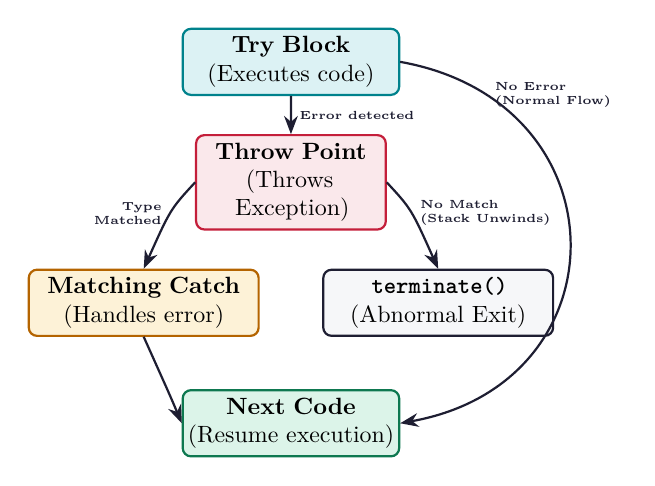
\begin{tikzpicture}[node distance=1.5cm, thick, scale=0.85, every node/.style={scale=0.85}]
  % Blocks
  \node[rectangle, draw=myteal, fill=hdrteal, rounded corners=3pt, text width=3.0cm, align=center, minimum height=0.8cm] (try) at (0, 2.4) {\textbf{Try Block} \\ (Executes code)};
  
  \node[rectangle, draw=myred, fill=hdrred, rounded corners=3pt, text width=2.6cm, align=center, minimum height=0.8cm] (throw) at (0, 0.6) {\textbf{Throw Point} \\ (Throws Exception)};
  
  \node[rectangle, draw=myamber, fill=hdramber, rounded corners=3pt, text width=3.2cm, align=center, minimum height=0.8cm] (catch) at (-2.2, -1.2) {\textbf{Matching Catch} \\ (Handles error)};
  
  \node[rectangle, draw=mydark, fill=mygray, rounded corners=3pt, text width=3.2cm, align=center, minimum height=0.8cm] (terminate) at (2.2, -1.2) {\textbf{\texttt{terminate()}} \\ (Abnormal Exit)};

  \node[rectangle, draw=mygreen, fill=hdrgreen, rounded corners=3pt, text width=3.0cm, align=center, minimum height=0.8cm] (next) at (0, -3.0) {\textbf{Next Code} \\ (Resume execution)};

  % Flows
  \draw[arrow] (try) -- (throw) node[midway, right, font=\tiny\bfseries\color{myred}] {Error detected};
  
  \draw[arrow] (throw.west) .. controls (-1.8, 0.2) .. (catch.north) node[midway, left, font=\tiny\bfseries\color{myteal}, align=right] {Type\\Matched};
  
  \draw[arrow] (throw.east) .. controls (1.8, 0.2) .. (terminate.north) node[midway, right, font=\tiny\bfseries\color{myamber}, align=left] {No Match\\(Stack Unwinds)};
  
  \draw[arrow] (catch.south) .. controls (-1.8, -2.6) .. (next.west);
  
  \draw[arrow] (try.east) .. controls (5.0, 1.8) and (5.0, -2.4) .. (next.east) node[pos=0.15, right, font=\tiny\bfseries\color{mygreen}, align=left] {No Error\\(Normal Flow)};
\end{tikzpicture}
\tcbset{colbacktitle=mgframe, coltitle=mydark}
\end{tcolorbox}

\begin{tcolorbox}[examplebox, title={Code Example: Exception throw point outside the main try block}]
\begin{spacing}{1.0}
\begin{verbatim}
#include <iostream>
// Function that throws exception
double divide(double a, double b) {
    if(b == 0.0) {
        throw "Division by zero condition!"; // Throws a const char*
    }
    return a / b;
}

int main() {
    double x = 10, y = 0, result;
    try {
        result = divide(x, y); // Throw point is inside divide()
        std::cout << "Result = " << result << std::endl;
    }
    catch(const char* msg) { // Catches the thrown char*
        std::cerr << "Caught Exception: " << msg << std::endl;
    }
    return 0;
}
\end{verbatim}
\end{spacing}
\tcbset{colbacktitle=myamber, coltitle=white}
\end{tcolorbox}

\subsection{Multiple Catches, Catch-All, and Re-throwing}
\begin{itemize}[leftmargin=*, itemsep=3pt]
  \item \textbf{Multiple Catches:} A single try block can have multiple sequential catch handlers to process different exception types.
  \item \textbf{Catch-All (\texttt{catch(...)}):} A special catch handler that intercepts any exception type. It must be placed at the very end of the handler list.
  \item \textbf{Exception Re-throwing:} An caught exception can be re-thrown using the \texttt{throw;} statement without arguments inside the catch block to pass it up to a higher scope.
\end{itemize}

% ===============================================================================
\section{Generic Programming using Templates}
% ===============================================================================

Templates allow writing code that is independent of data types, enabling the creation of generic functions and classes.

\subsection{Function Templates}
Function templates act as formulas for generating functions based on argument types.
\begin{tcolorbox}[formulabox, title={\textbf{Function Template Syntax}}]
\begin{equation}
  \texttt{template <typename T> } \quad \text{Return\_Type} \quad \text{FuncName}(\text{T args}) \quad \{ \dots \}
\end{equation}
\end{tcolorbox}

\begin{tcolorbox}[examplebox, title={Code Example: Multi-parameter function template}]
\begin{spacing}{1.0}
\begin{verbatim}
#include <iostream>
// Multi-parameter function template
template <typename T1, typename T2>
void printComparison(T1 x, T2 y) {
    if(x > y) {
        std::cout << x << " is larger than " << y << std::endl;
    } else {
        std::cout << x << " is not larger than " << y << std::endl;
    }
}

int main() {
    printComparison(10, 5.5); // T1 = int, T2 = double
    printComparison(4.2, 9.8); // T1 = double, T2 = double
    return 0;
}
\end{verbatim}
\end{spacing}
\tcbset{colbacktitle=myamber, coltitle=white}
\end{tcolorbox}

\subsection{Class Templates}
Class templates are used to create generic containers or data structures that operate on any data type.
\begin{tcolorbox}[examplebox, title={Code Example: Generic Stack class template}]
\begin{spacing}{1.0}
\begin{verbatim}
#include <iostream>
template <typename T, int SIZE = 10> // typename T and non-type int SIZE
class Stack {
private:
    T arr[SIZE];
    int top;
public:
    Stack() : top(-1) {}
    
    bool push(T element) {
        if(top >= SIZE - 1) return false; // Overflow
        arr[++top] = element;
        return true;
    }
    
    T pop() {
        if(top < 0) throw "Stack Underflow!"; // Throw const char*
        return arr[top--];
    }
};

int main() {
    try {
        Stack<int, 5> intStack; // Instantiate an int stack of size 5
        intStack.push(10);
        intStack.push(20);
        std::cout << intStack.pop() << std::endl; // 20
        std::cout << intStack.pop() << std::endl; // 10
        std::cout << intStack.pop() << std::endl; // Throws exception
    }
    catch(const char* e) {
        std::cout << "Exception: " << e << std::endl;
    }
    return 0;
}
\end{verbatim}
\end{spacing}
\tcbset{colbacktitle=myamber, coltitle=white}
\end{tcolorbox}

% ===============================================================================
% MANDATORY QUICK REVISION PAGE
% ===============================================================================
\newpage
\begin{center}
  {\large\bfseries\color{myred} Quick Revision --- Module IX}\\[3pt]
  {\small\color{mydark} Exception Handling \& Templates $|$ OE-EC604C}
\end{center}
\noindent{\color{myred}\rule{\linewidth}{1.2pt}}
\vspace{4pt}

\begin{tcolorbox}[formulabox, title={\textbf{Key Exception and Template Syntax}}]
\renewcommand{\arraystretch}{1.3}
\begin{tabularx}{\linewidth}{B{3.8cm} X}
Try-Catch Block          & \texttt{try \{ throw 404; \} catch(int err) \{ /* handles 404 */ \}} \\[4pt]
Catch-All Handler        & \texttt{catch(...) \{ /* catches any exception type */ \}} \\[4pt]
Re-throwing              & \texttt{catch(const char* e) \{ throw; // Re-throws exception up \} } \\[4pt]
Function Template        & \texttt{template <typename T> T maxVal(T a, T b) \{ return (a > b) ? a : b; \}} \\[4pt]
Class Template           & \texttt{template <class T> class Box \{ T value; \};} \\[4pt]
Template Instantiation   & \texttt{Box<double> doubleBox; // Explicit template argument}
\end{tabularx}
\end{tcolorbox}

\begin{tcolorbox}[defbox, title={\textbf{One-Line Definitions}}]
\begin{itemize}[leftmargin=*, itemsep=2.5pt, topsep=0pt]
  \item \textbf{Exception:} A runtime error or anomaly that disrupts the normal execution flow of a program.
  \item \textbf{Stack Unwinding:} The automatic destruction of local variables in stack frames during exception propagation.
  \item \textbf{Catch-All Handler:} A fallback handler (\texttt{catch(...)}) that catches any exception type not previously intercepted.
  \item \textbf{Re-throwing:} Forwarding an caught exception up to the parent calling frame using the \texttt{throw;} statement.
  \item \textbf{Template:} A blueprint used by the compiler to generate type-specific functions or classes automatically.
  \item \textbf{Generic Programming:} A programming model focused on writing algorithms independent of specific data types.
  \item \textbf{Non-type Template Parameter:} A template parameter that represents a constant value (e.g., \texttt{int SIZE}) rather than a type.
  \item \textbf{Template Specialization:} Defining a unique template implementation for a specific data type (e.g., \texttt{T = char*}).
  \item \textbf{terminate():} A system function called when no matching catch handler is found for a thrown exception.
\end{itemize}
\end{tcolorbox}

\begin{tcolorbox}[exambox, title={\textbf{Frequently Asked / Viva Questions}}]
\begin{enumerate}[topsep=0pt, label=\textbf{Q\arabic*.}, itemsep=5pt]
  \item \Q{What happens if an exception is thrown but no matching catch block is found?}
    The runtime library calls the `terminate()` function, which by default calls `abort()` to terminate the program immediately.
  \item \Q{Can we throw class objects as exceptions in C++?}
    Yes. Throwing class instances is the standard way to implement custom exceptions, allowing structured error data to be passed to handlers.
  \item \Q{What is the purpose of the catch-all handler and where must it be placed?}
    `catch(...)` catches all exception types. It acts as a safety net and must be placed as the last handler, otherwise it blocks subsequent handlers.
  \item \Q{Why does template instantiation not happen at class definition time?}
    A template only defines a blueprint. The compiler only generates class code when the template is instantiated with a specific type (e.g., `Stack<int>`).
  \item \Q{Explain the compile-time overhead associated with templates.}
    Templates require the compiler to generate unique code for each type instantiation, which increases compile times and binary sizes (code bloat).
  \item \Q{What is template function specialization?}
    It allows defining a custom implementation of a function template for a specific data type (e.g., optimizing string comparisons instead of pointer comparisons).
  \item \Q{Can templates have default arguments?}
    Yes. Both class templates and function templates (in C++11) can have default type arguments (e.g., `template <typename T = int>`).
  \item \Q{How does the compiler select between overloaded template functions and regular functions?}
    The compiler prefers a regular non-template function if it matches the arguments exactly. If no match is found, it instantiates the template.
  \item \Q{Explain the difference between exception handling in C++ vs. Java.}
    C++ does not support checked exceptions (you do not have to declare exceptions in method signatures), and it does not have a native `finally` block (resource cleanup relies on RAII).
  \item \Q{What is the difference between `typename` and `class` keywords in template declarations?}
    Inside template parameters, `typename` and `class` are completely equivalent and interchangeable. E.g., `template <class T>` and `template <typename T>` behave identically.
  \item \Q{Why is it dangerous to throw pointers to local variables?}
    Local variables are destroyed when stack frames are unwound. The handler will receive a dangling pointer to invalid memory, causing undefined behavior.
  \item \Q{What is the RAII (Resource Acquisition Is Initialization) pattern?}
    It is a design pattern where resources (files, memory, locks) are bound to the lifetime of local objects. Destructors automatically release resources during normal exit or stack unwinding, preventing leaks.
\end{enumerate}
\tcbset{colbacktitle=mypurple, coltitle=white}
\end{tcolorbox}

\begin{tcolorbox}[tikzbox, title={Comparison: Exception Handling vs. Traditional Error Return Codes}]
\renewcommand{\arraystretch}{1.45}
\par\noindent
\begin{tabularx}{\linewidth}{|B{3.2cm}|Y|Y|}
\hline
\textbf{Feature} & \textbf{\color{myteal}Exception Handling (try-catch)} & \textbf{\color{myamber}Traditional Error Codes (if-else)} \\
\hline
\textbf{Separation} & Clear separation between execution logic and error handling code. & Error checking logic is mixed directly into the main algorithm. \\
\hline
\textbf{Propagation} & Errors propagate automatically up the call stack until handled. & Errors must be explicitly returned and checked in every function frame. \\
\hline
\textbf{Data Payload} & Exceptions can pass complex objects containing detailed error info. & Limited to returning simple integer codes or status booleans. \\
\hline
\textbf{Performance} & Slower when exceptions occur (due to stack unwinding and V-Table lookup). & Minimal overhead (simple conditional branches). \\
\hline
\textbf{Uncaught Errors} & Leads to immediate program termination (safe fail-fast). & Can be silently ignored, causing latent bugs or data corruption. \\
\hline
\end{tabularx}
\tcbset{colbacktitle=mgframe, coltitle=mydark}
\end{tcolorbox}


\end{document}
